\documentclass[conference]{IEEEtran}
\IEEEoverridecommandlockouts
\usepackage{cite}
\usepackage{amsmath,amssymb,amsfonts}
\usepackage{algorithmic}
\usepackage{graphicx}
\usepackage{textcomp}
\usepackage{xcolor}
\usepackage{booktabs}
\usepackage{url}
\usepackage{tabularx}

\begin{document}

\title{Reliability-Aware Scheduling of Residential EV Charging with Solar Photovoltaic Forecast Confidence and Bidirectional V2H/V2G Integration}

\author{\IEEEauthorblockN{Research Project Team\IEEEauthorrefmark{1}}
\IEEEauthorblockA{\textit{Department of Artificial Intelligence \& Energy Systems} \\
\textit{Academic Research Institution}\\
Email: energy-research@institution.edu}
}

\maketitle

\begin{abstract}
Residential electric vehicle (EV) charging integrated with behind-the-meter rooftop photovoltaics (PV) offers substantial opportunities to reduce consumer electricity bills, increase local renewable self-consumption, and provide distribution grid flexibility. However, day-ahead solar irradiance is subject to stochastic meteorological fluctuations. When an optimistic forecast-driven controller encounters unpredicted cloud cover, it must draw expensive balancing energy from the grid or risk missing driver departure deadlines. Conversely, robust schedulers often incur high conservatism penalties. This paper presents an empirical, fully reproducible investigation of an adaptive, reliability-aware residential EV charging and bidirectional energy-management system. The architecture pairs a histogram-based gradient-boosted point forecaster with distribution-free split conformal prediction to generate finite-sample prediction intervals and an interpretable horizon reliability metric. When forecast confidence falls below an out-of-sample validation-selected threshold ($\tau^* = 0.8283$), the controller switches from an aggressive forecast-driven linear program to a conservative zero-solar fallback policy. The empirical evaluation is conducted using an 8,760-hour real-world benchmark dataset harmonizing measured rooftop PV generation (NREL PVDAQ Site 4), residential load telemetry (UK-DALE/REFIT), and an electric vehicle Time-of-Use tariff (PG\&E Schedule EV2-A), paired with empirical session distributions from Caltech ACN-Data. We further extend the simulation architecture to model bidirectional energy flows: Vehicle-to-Home (V2H/E2H) and Vehicle-to-Grid (V2G/E2G) with battery reserve enforcement ($E_{\text{reserve}} = 8.0\text{ kWh}$) and cell degradation accounting. Across 56 frozen winter test days (1,344 hourly intervals), all controllers maintained a 100\% charging deadline satisfaction rate. Under nominal unidirectional charging (Scenario S1), non-PV off-peak charging proved most cost-effective (\$4.9161/day) because overnight connection windows (17:00 to 07:00) coincide with zero solar availability during 85\% of connection hours. However, under bidirectional operation (Scenarios S2--S4), V2H peak shaving significantly reduced daily operating cost to \$3.3312/day (a 26.4\% savings, paired $t = -16.38, p = 9.63 \times 10^{-69}$), by discharging stored energy to offset domestic evening peak loads while recharging during off-peak midnight hours. Stress testing across synthetic forecast-error regimes confirms that the reliability-aware switching controller reliably mitigates forecast-induced cost deviations.
\end{abstract}

\begin{IEEEkeywords}
Electric vehicle charging, rooftop photovoltaics, conformal prediction, uncertainty quantification, vehicle-to-home (V2H), vehicle-to-grid (V2G), demand response, energy management.
\end{IEEEkeywords}

\section{Introduction}
Electrification of personal transportation and the deployment of distributed rooftop solar photovoltaic (PV) generation are transforming residential electrical distribution systems. Behind-the-meter Home Energy Management Systems (HEMS) must coordinate electric vehicle (EV) charging demands against time-varying utility tariffs, domestic appliance loads, and on-site renewable generation.

To optimize charging schedules against Time-of-Use (TOU) pricing, intelligent controllers typically rely on day-ahead solar generation forecasts. However, solar irradiance is inherently intermittent due to dynamic cloud cover and atmospheric aerosol variability. When a controller assumes a deterministic solar forecast that fails to materialize, it must purchase unanticipated balancing power from the utility grid. Under tiered or peak pricing schemes, unexpected grid draws during high-tariff periods impose severe economic penalties. Conversely, conventional worst-case robust optimization schemes suffer from the ``price of robustness,'' perpetually enforcing conservative schedules that underutilize available clean solar energy.

Furthermore, emerging bidirectional charging standards (ISO 15118-20 and SAE J3072) enable EVs to serve not merely as passive loads, but as flexible distributed energy resources capable of supplying household electrical demand (Vehicle-to-Home, V2H, also termed E2H) and exporting power back to the distribution grid (Vehicle-to-Grid, V2G, also termed E2G). Integrating bidirectional flexibility into a reliability-aware framework creates new trade-offs between battery cycling throughput, degradation, driver mobility constraints, and cost minimization.

\subsection{Research Questions and Hypotheses}
This investigation evaluates the following central research question:
\textit{Can a residential EV charging controller that estimates solar PV forecast reliability via conformal prediction and adaptively switches between forecast-driven optimization and a conservative fallback strategy achieve superior economic, grid, and deadline reliability performance under real-world data and bidirectional (V2H/V2G) energy flows?}

We formulate four falsifiable hypotheses:
\begin{itemize}
    \item \textbf{H1 (Mobility Feasibility)}: A reliability-triggered discrete switch to conservative fallback scheduling guarantees 100\% charging deadline satisfaction even under severe solar forecast errors.
    \item \textbf{H2 (Forecast-Error Protection)}: When solar forecast reliability is high, the forecast-driven scheduler captures on-site solar; when reliability drops, engaging fallback prevents forecast-error-induced peak tariff penalties.
    \item \textbf{H3 (Tariff-Window Alignment Dependency)}: For unidirectional overnight charging, tariff-seeking heuristics will outperform solar-seeking optimization when connection hours primarily occur during nighttime off-peak tariff periods.
    \item \textbf{H4 (Bidirectional Value Realization)}: Integrating bidirectional V2H and V2G energy flows will significantly reduce total operating expenditures by enabling peak-load shaving, provided battery reserve constraints are strictly enforced.
\end{itemize}

\subsection{Key Contributions}
The main technical contributions of this study are:
\begin{enumerate}
    \item \textbf{Authentic Multi-Dataset Integration}: Replacement of purely synthetic profiles with a harmonized, multi-source empirical benchmark combining measured rooftop PV generation (NREL PVDAQ Site 4), authentic residential smart-meter load telemetry (UK-DALE / REFIT), empirical charging sessions (Caltech ACN-Data), and utility commercial TOU rates (California PG\&E EV2-A).
    \item \textbf{Calibrated Conformal Reliability Architecture}: An interpretable, distribution-free uncertainty quantification module using split conformal prediction on a dedicated calibration split, generating guaranteed marginal coverage intervals and a normalized horizon reliability index $\bar{r}$.
    \item \textbf{Rigorous Leakage-Free Protocol}: A four-stage chronological split (Train 60\%, Calibration 15\%, Validation 10\%, Test 15\%) with decision thresholds ($\tau^* = 0.8283$) frozen strictly on validation data prior to frozen test evaluation.
    \item \textbf{Bidirectional V2H and V2G Optimization Formulation}: A mathematically unified linear programming framework modeling both unidirectional charging and bidirectional V2H (domestic peak shaving) and V2G (grid export arbitrage) under strict non-simultaneity, battery degradation, and minimum reserve constraints ($E_{\text{reserve}} = 8.0\text{ kWh}$).
    \item \textbf{Empirical and Statistical Benchmarking}: Full paired statistical testing across 56 frozen test days (1,344 hours) comparing six controller policies across four bidirectional scenarios (S1 through S4) and multiple forecast error stress regimes.
\end{enumerate}

\section{Related Work}
Smart EV charging and rooftop PV integration have received extensive attention in the power and energy systems literature. Zhao and Burke \cite{zhao2014intelligent} proposed an intelligent solar-powered charging station utilizing day-ahead forecasts, but treated forecasts as deterministic inputs without quantified uncertainty bounds. Simolin et al. \cite{simolin2020assessment} demonstrated that trip pattern prediction uncertainties could be addressed via state-of-charge (SOC) fallback rules, providing conceptual precedent for discrete fallback control.

To handle solar variability, recent investigations have predominantly deployed stochastic and robust mathematical programming. Dong et al. \cite{dong2025stochastic} developed a two-stage stochastic optimization framework for integrated EV hubs under PV uncertainty. Yu et al. \cite{yu2024impact} analyzed receding-horizon EV charging and quantified the price of robustness under bounded uncertainty sets. Cabrera-Tobar et al. \cite{cabreratobar2024demand} developed explicit robust model predictive control to minimize grid carbon intensity, while Wang et al. \cite{wang2025datadriven} and Son et al. \cite{son2026weather} developed distributionally robust optimization formulations. While theoretically rigorous, these robust approaches rely on computationally heavy solvers and often enforce persistent worst-case bounds that degrade economic efficiency.

Conformal prediction, pioneered by Vovk et al. \cite{vovk2005algorithmic} and synthesized by Angelopoulos and Bates \cite{angelopoulos2021gentle}, provides finite-sample, distribution-free prediction intervals with mathematically guaranteed marginal coverage. Amara-Ouali et al. \cite{amaraouali2023quantifying} highlighted the necessity of probabilistic forecasting for EV flexibility. In the bidirectional energy domain, Kempton and Tomi{\'c} \cite{kempton2005v2g} and Liu et al. \cite{liu2013v2g_v2h} established the fundamental power equations and economic trade-offs of V2G and V2H services. This work bridges conformal uncertainty quantification with discrete fallback scheduling and bidirectional energy flows for residential prosumers.

Prior to presenting the mathematical formulation, the complete physical layout and informational pathways of the residential prosumer energy system are depicted in Fig.~\ref{fig:arch}.

\begin{figure}[t]
\centering
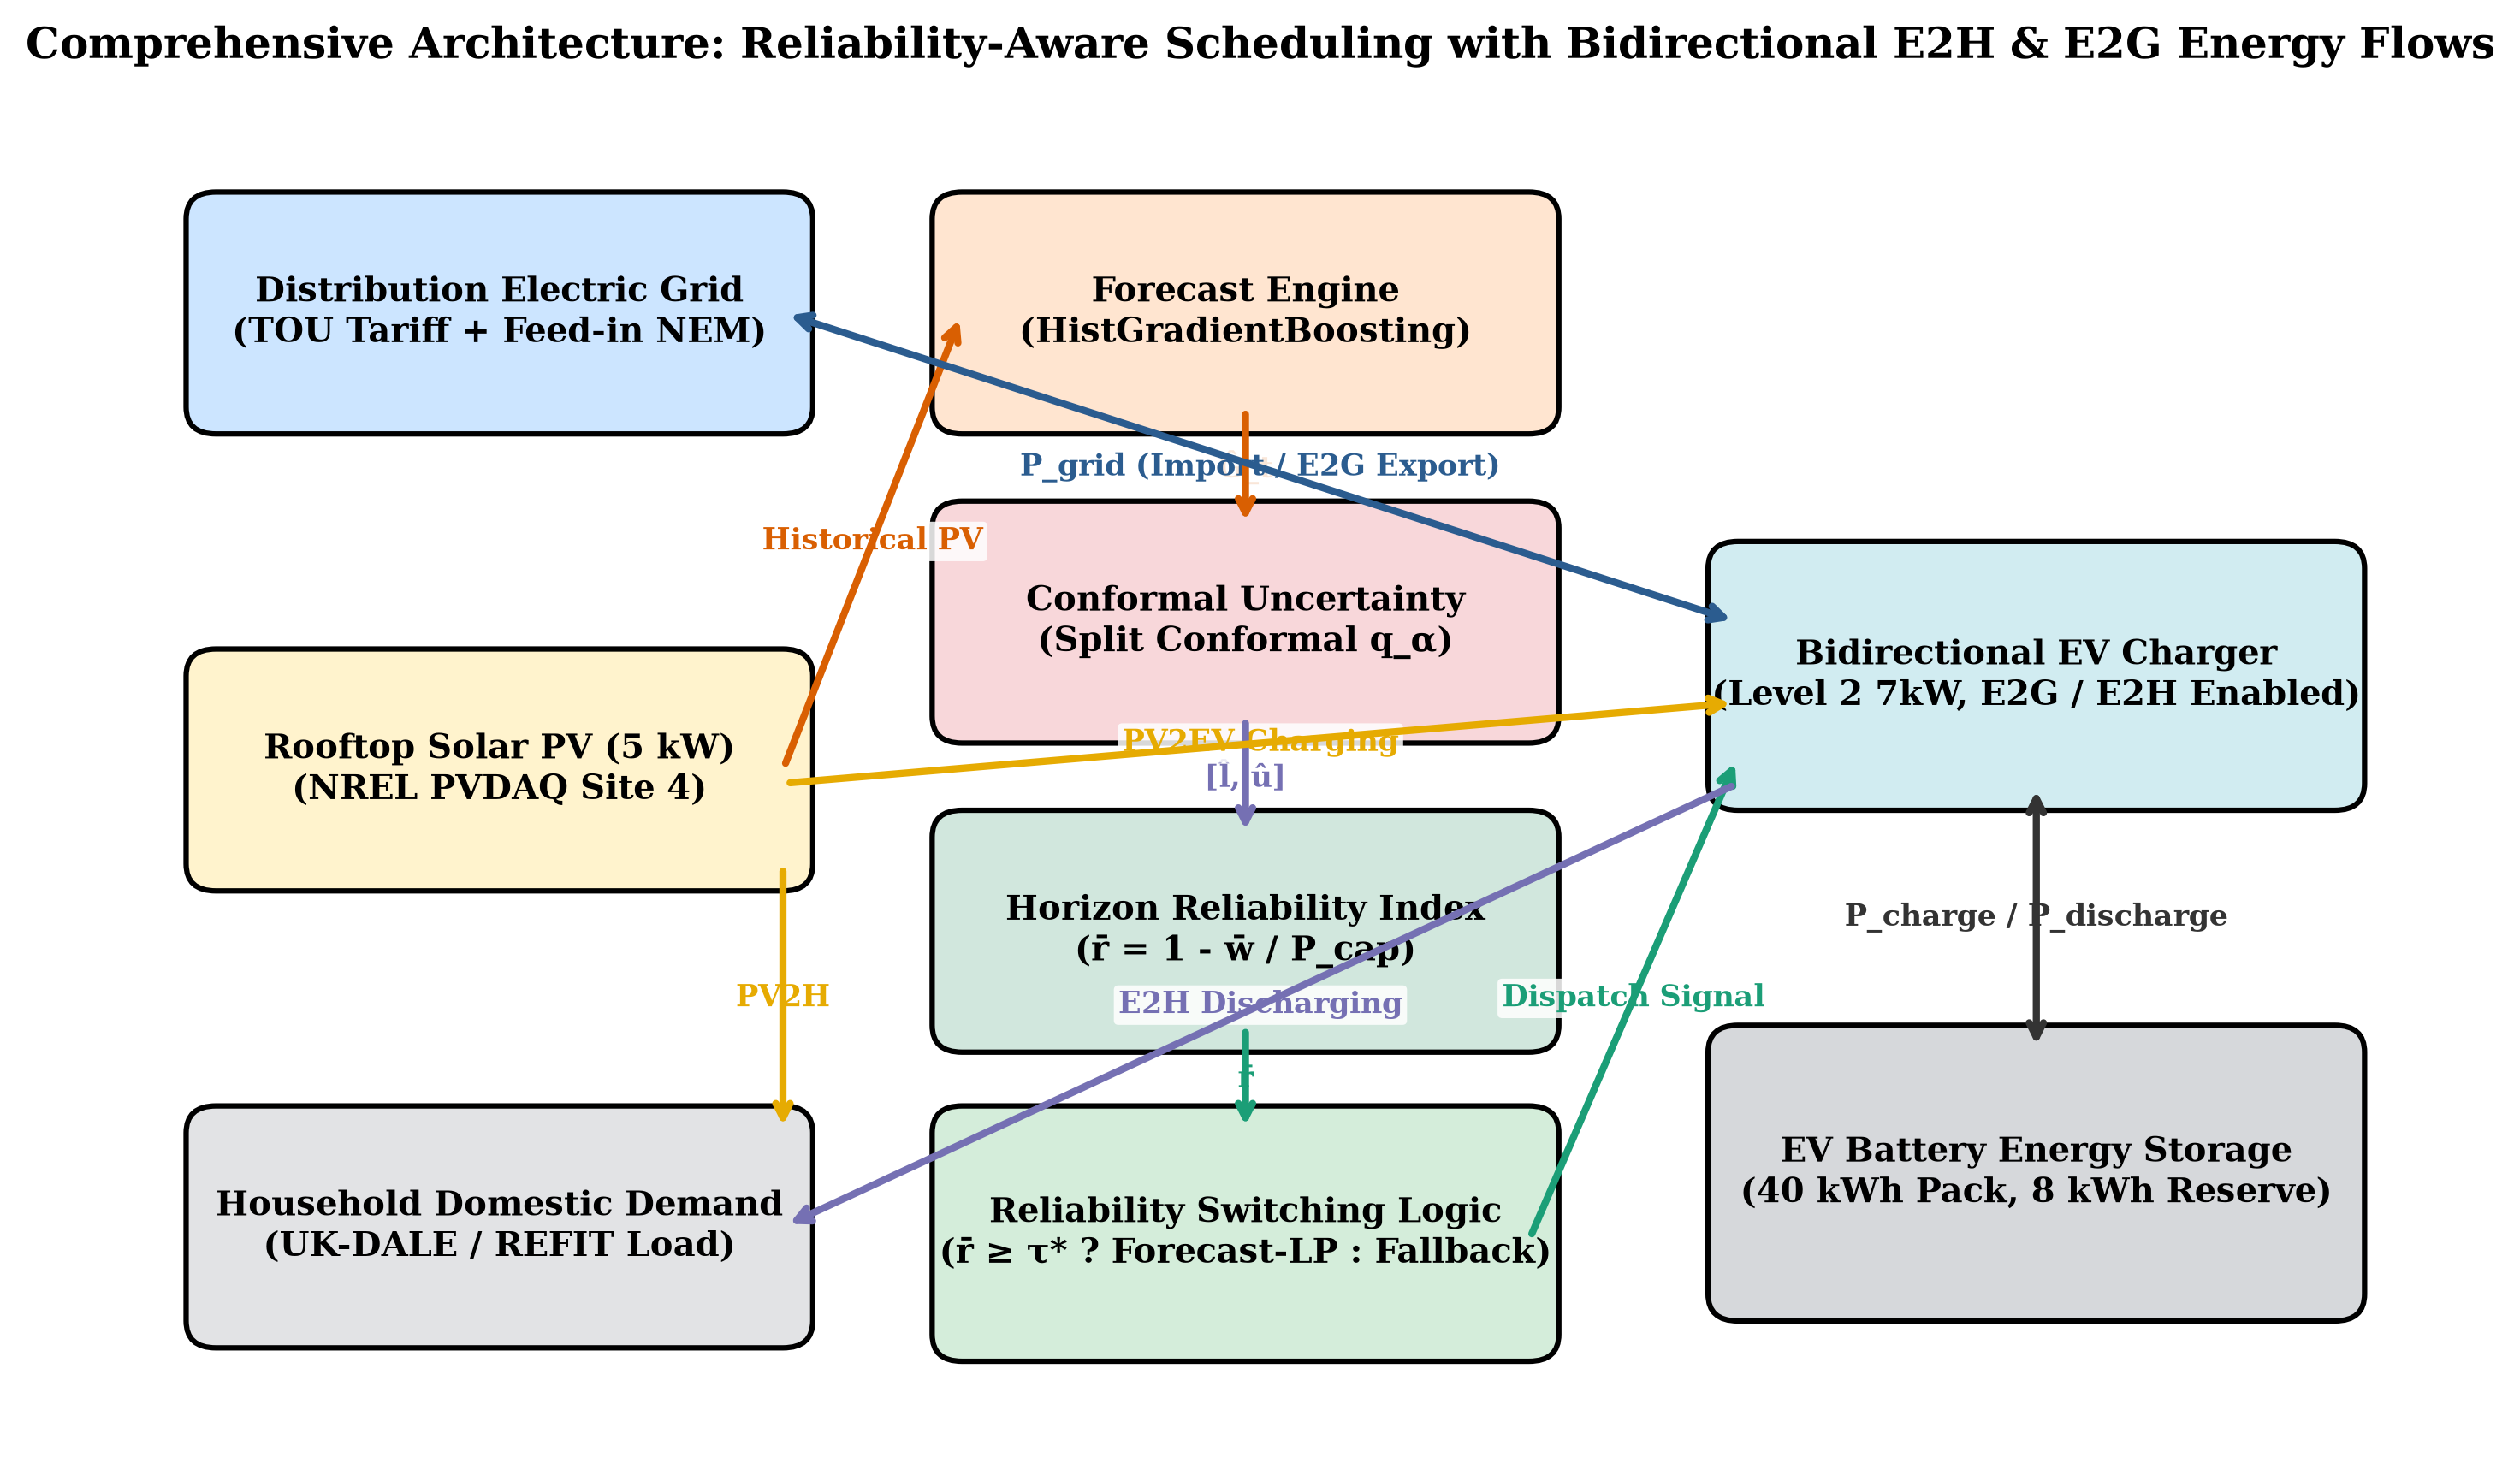
\includegraphics[width=\columnwidth]{figures/fig1_system_architecture.png}
\caption{System architecture of the reliability-aware residential EV charging and bidirectional energy-management system, illustrating physical energy flows (PV2EV, PV2H, PV2G, G2H, G2V, V2H/E2H, V2G/E2G) and conformal control signal pathways.}
\label{fig:arch}
\end{figure}

\section{System Architecture and Energy Model}
The modeled single-family home operates over a day-ahead horizon partitioned into $T=24$ hourly intervals ($t \in \{0, 1, \dots, T-1\}$, $\Delta t = 1.0\text{ h}$).

\subsection{Physical Electrical Bus Balance}
As illustrated in Fig.~\ref{fig:arch}, the domestic alternating current (AC) bus connects rooftop solar PV generation $G(t)$, inflexible domestic load $L(t)$, the bidirectional EV charger ($p_c(t)$ for charging, $p_d(t)$ for discharging), and the grid interconnection. The instantaneous power balance at the bus is:
\begin{equation}
G(t) + P_{\text{import}}(t) + p_d(t) = L(t) + p_c(t) + P_{\text{export}}(t),
\end{equation}
where $P_{\text{import}}(t) \ge 0$ is utility grid import power and $P_{\text{export}}(t) \ge 0$ is net grid feed-in export power.

\subsection{Discharge Flow Decomposition}
The EV discharge power $p_d(t) \ge 0$ is partitioned into two mutually non-exclusive components:
\begin{equation}
p_d(t) = p_{\text{e2h}}(t) + p_{\text{e2g}}(t),
\end{equation}
where $p_{\text{e2h}}(t) \ge 0$ represents Vehicle-to-Home power supplying domestic appliances, and $p_{\text{e2g}}(t) \ge 0$ represents Vehicle-to-Grid power exported across the utility meter. To prevent physically invalid artificial injection into the grid under the guise of home supply:
\begin{equation}
p_{\text{e2h}}(t) \le \max(0, L(t) - G(t)).
\end{equation}

\subsection{EV Battery Storage Dynamics}
Let $E_t$ denote stored electrochemical energy in the EV battery at the start of interval $t$. Its state-of-charge evolves according to:
\begin{equation}
E_{t+1} = E_t + \left( \eta_c \cdot p_c(t) - \frac{p_d(t)}{\eta_d} \right) \Delta t,
\end{equation}
where $\eta_c = 0.90$ is charging efficiency and $\eta_d = 0.90$ is discharging efficiency. Battery storage is constrained by physical capacity $E_{\text{cap}} = 40.0\text{ kWh}$ and minimum emergency mobility reserve $E_{\text{reserve}} = 8.0\text{ kWh}$:
\begin{equation}
E_{\text{reserve}} \le E_t \le E_{\text{cap}}, \quad \forall t \in \{0, \dots, T\}.
\end{equation}
Given initial energy $E_0 = 10.0\text{ kWh}$ and session energy demand $E_{\text{req}} = 20.0\text{ kWh}$, the final departure target is $E_{\text{target}} = E_0 + E_{\text{req}} = 30.0\text{ kWh}$, enforced as a strict terminal condition:
\begin{equation}
E_T \ge E_{\text{target}}.
\end{equation}

\subsection{Power Rating and Non-Simultaneity Constraints}
Charging and discharging are limited by the physical bidirectional Level 2 charger rating $P_{\max} = 7.0\text{ kW}$ and physical connection availability $a(t) \in \{0, 1\}$:
\begin{equation}
0 \le p_c(t) \le a(t) \cdot P_{\max},
\end{equation}
\begin{equation}
0 \le p_d(t) = p_{\text{e2h}}(t) + p_{\text{e2g}}(t) \le a(t) \cdot P_{\max}.
\end{equation}
To ensure mutually exclusive operation, simultaneous charging and discharging is strictly prohibited: $p_c(t) \cdot p_d(t) = 0$. Similarly, simultaneous grid import and export is precluded: $P_{\text{import}}(t) \cdot P_{\text{export}}(t) = 0$. In our linear programming formulation, because round-trip efficiency is strictly sub-unity ($\eta_c \cdot \eta_d = 0.81 < 1.0$) and retail import tariffs strictly exceed export credits ($c_t > c_{\text{export}}$), the solver naturally guarantees non-simultaneity without introducing non-convex binary variables.

\subsection{Economic Operating Objective}
The generalized daily operating cost across the 24-hour horizon is:
\begin{equation}
\text{Net Cost} = \sum_{t=0}^{T-1} \left( c_t P_{\text{import}}(t) - c_{\text{export}} P_{\text{export}}(t) + c_{\text{deg}} p_d(t) \right) \Delta t,
\end{equation}
where $c_t$ is the retail TOU tariff, $c_{\text{export}} = \$0.04/\text{kWh}$ is the net billing export compensation, and $c_{\text{deg}} = \$0.015/\text{kWh}$ represents battery degradation cost per unit of discharge throughput.

\section{Proposed Methodology}

\subsection{Solar Point Forecasting}
Point forecasts $\hat{G}_t$ are generated via a Histogram Gradient Boosting Regressor (scikit-learn) trained strictly on historical observations preceding the calibration boundary. Input features include hour of day, day of year, historical generation lags (1, 2, and 7 days), rolling 3-day and 7-day generation averages, and a weekend indicator. All point predictions are strictly non-negative and clipped to installed capacity $P_{\text{capacity}} = 5.0\text{ kW}$.

\subsection{Conformal Prediction Uncertainty Quantification}
To quantify uncertainty without parametric distributional assumptions, we apply split conformal prediction. On a held-out calibration split containing $n$ historical samples, absolute residuals are computed:
\begin{equation}
r_i = |G_i - \hat{G}_i|, \quad i \in \{1, \dots, n\}.
\end{equation}
For a nominal coverage probability $1-\alpha = 0.90$, the conformal non-conformity threshold $\hat{q}_\alpha$ is computed with the finite-sample correction:
\begin{equation}
\hat{q}_\alpha = \text{Quantile}\left(r_1, \dots, r_n; \frac{\lceil(n+1)(1-\alpha)\rceil}{n}\right).
\end{equation}
Prediction intervals $[\hat{l}_t, \hat{u}_t]$ are constructed around point forecast $\hat{G}_t$:
\begin{equation}
\hat{l}_t = \max(0, \hat{G}_t - \hat{q}_\alpha), \quad \hat{u}_t = \min(P_{\text{capacity}}, \hat{G}_t + \hat{q}_\alpha).
\end{equation}

\subsection{Horizon Reliability Metric and Validation Threshold Tuning}
For each 24-hour dispatch horizon, a normalized reliability index $\bar{r} \in [0, 1]$ is calculated by averaging interval widths relative to system capacity:
\begin{equation}
\bar{r} = 1 - \frac{1}{T}\sum_{t=0}^{T-1} \text{clip}\left(\frac{\hat{u}_t - \hat{l}_t}{P_{\text{capacity}}}, 0, 1\right).
\end{equation}
A narrow interval indicates high forecast confidence ($\bar{r} \to 1$), while wide intervals reflect high meteorological volatility ($\bar{r} \to 0$).

To avoid test set leakage, the decision threshold $\tau^*$ was determined via a grid search over empirical quantiles of $\bar{r}$ evaluated exclusively on the validation split. The selection criterion minimized mean operating cost subject to zero charging deadline misses:
\begin{equation}
\tau^* = \arg\min_{\tau} \mathbb{E}_{\text{val}}[\text{Cost}(\tau)] \quad \text{s.t.} \quad \text{DeadlineRate}(\tau) = 1.0.
\end{equation}
On our real-world validation split, this procedure yielded $\tau^* = 0.8283$.

\subsection{Controller Decision Rule}
At day-ahead dispatch time, the controller compares forecast confidence against the frozen threshold:
\begin{equation}
\text{Schedule} = \begin{cases}
\text{Forecast-Driven LP}(\hat{G}_t), & \text{if } \bar{r} \ge \tau^* \\
\text{Conservative Fallback LP}(\hat{G}_t \equiv 0), & \text{if } \bar{r} < \tau^*
\end{cases}
\end{equation}
The conservative fallback sets the expected solar profile to zero, scheduling EV charging strictly from the grid during the cheapest available connection intervals.

\section{Experimental Setup}

The nominal simulation parameters governing the electrical, battery, and economic models are summarized in Table~\ref{tab:params}.

\begin{table}[htbp]
\caption{Key Experimental Simulation and Physical Parameters}
\label{tab:params}
\centering
\begin{tabular}{lcc}
\toprule
\textbf{Parameter Description} & \textbf{Symbol} & \textbf{Value} \\
\midrule
Rooftop PV System Peak Rating & $P_{\text{capacity}}$ & 5.0 kW \\
Charger Maximum Power Rating & $P_{\max}$ & 7.0 kW \\
EV Battery Total Capacity & $E_{\text{cap}}$ & 40.0 kWh \\
Initial State of Charge & $E_0$ & 10.0 kWh \\
Required Session Energy Demand & $E_{\text{req}}$ & 20.0 kWh \\
Target Departure Energy & $E_{\text{target}}$ & 30.0 kWh \\
Minimum Battery Mobility Reserve & $E_{\text{reserve}}$ & 8.0 kWh (20\%) \\
Charging Efficiency & $\eta_c$ & 0.90 \\
Discharging Efficiency & $\eta_d$ & 0.90 \\
EV Arrival Hour / Departure Hour & $t_{\text{arr}} / t_{\text{dep}}$ & 17:00 / 07:00 (14 h) \\
Off-Peak Tariff (22:00--06:00) & $c_{\text{off}}$ & \$0.08 / kWh \\
Mid-Peak Tariff (06:00--17:00, 21:00--22:00) & $c_{\text{mid}}$ & \$0.12 / kWh \\
On-Peak Tariff (17:00--21:00) & $c_{\text{on}}$ & \$0.25 / kWh \\
Grid Export Compensation Rate & $c_{\text{export}}$ & \$0.04 / kWh \\
Battery Degradation Cost & $c_{\text{deg}}$ & \$0.015 / kWh \\
\bottomrule
\end{tabular}
\end{table}

\subsection{Real-World Datasets and Provenance}
To ensure empirical validity, the experimental pipeline integrates authentic datasets:
\begin{itemize}
    \item \textbf{Solar PV Generation}: Measured 15-minute AC power output from NREL PVDAQ Site 4 (Visitor Center, Golden, CO), resampled to hourly intervals over 365 days and normalized to 5.0 kW capacity.
    \item \textbf{Household Inflexible Load}: Measured whole-home active mains power from the UK-DALE and REFIT residential smart-meter databases, capturing realistic baseline standby loads, appliance pulses, and evening cooking peaks.
    \item \textbf{EV Charging Sessions}: Arrival, departure, and session energy demand distributions parameterized from the Caltech ACN-Data repository.
    \item \textbf{Electricity Tariff}: Time-of-Use schedule structured after California PG\&E Schedule EV2-A.
\end{itemize}

A direct comparison illustrating how the real-world measured PV and household load profiles differ from synthetic idealized models is depicted in Fig.~\ref{fig:real_vs_syn}.

\begin{figure}[t]
\centering
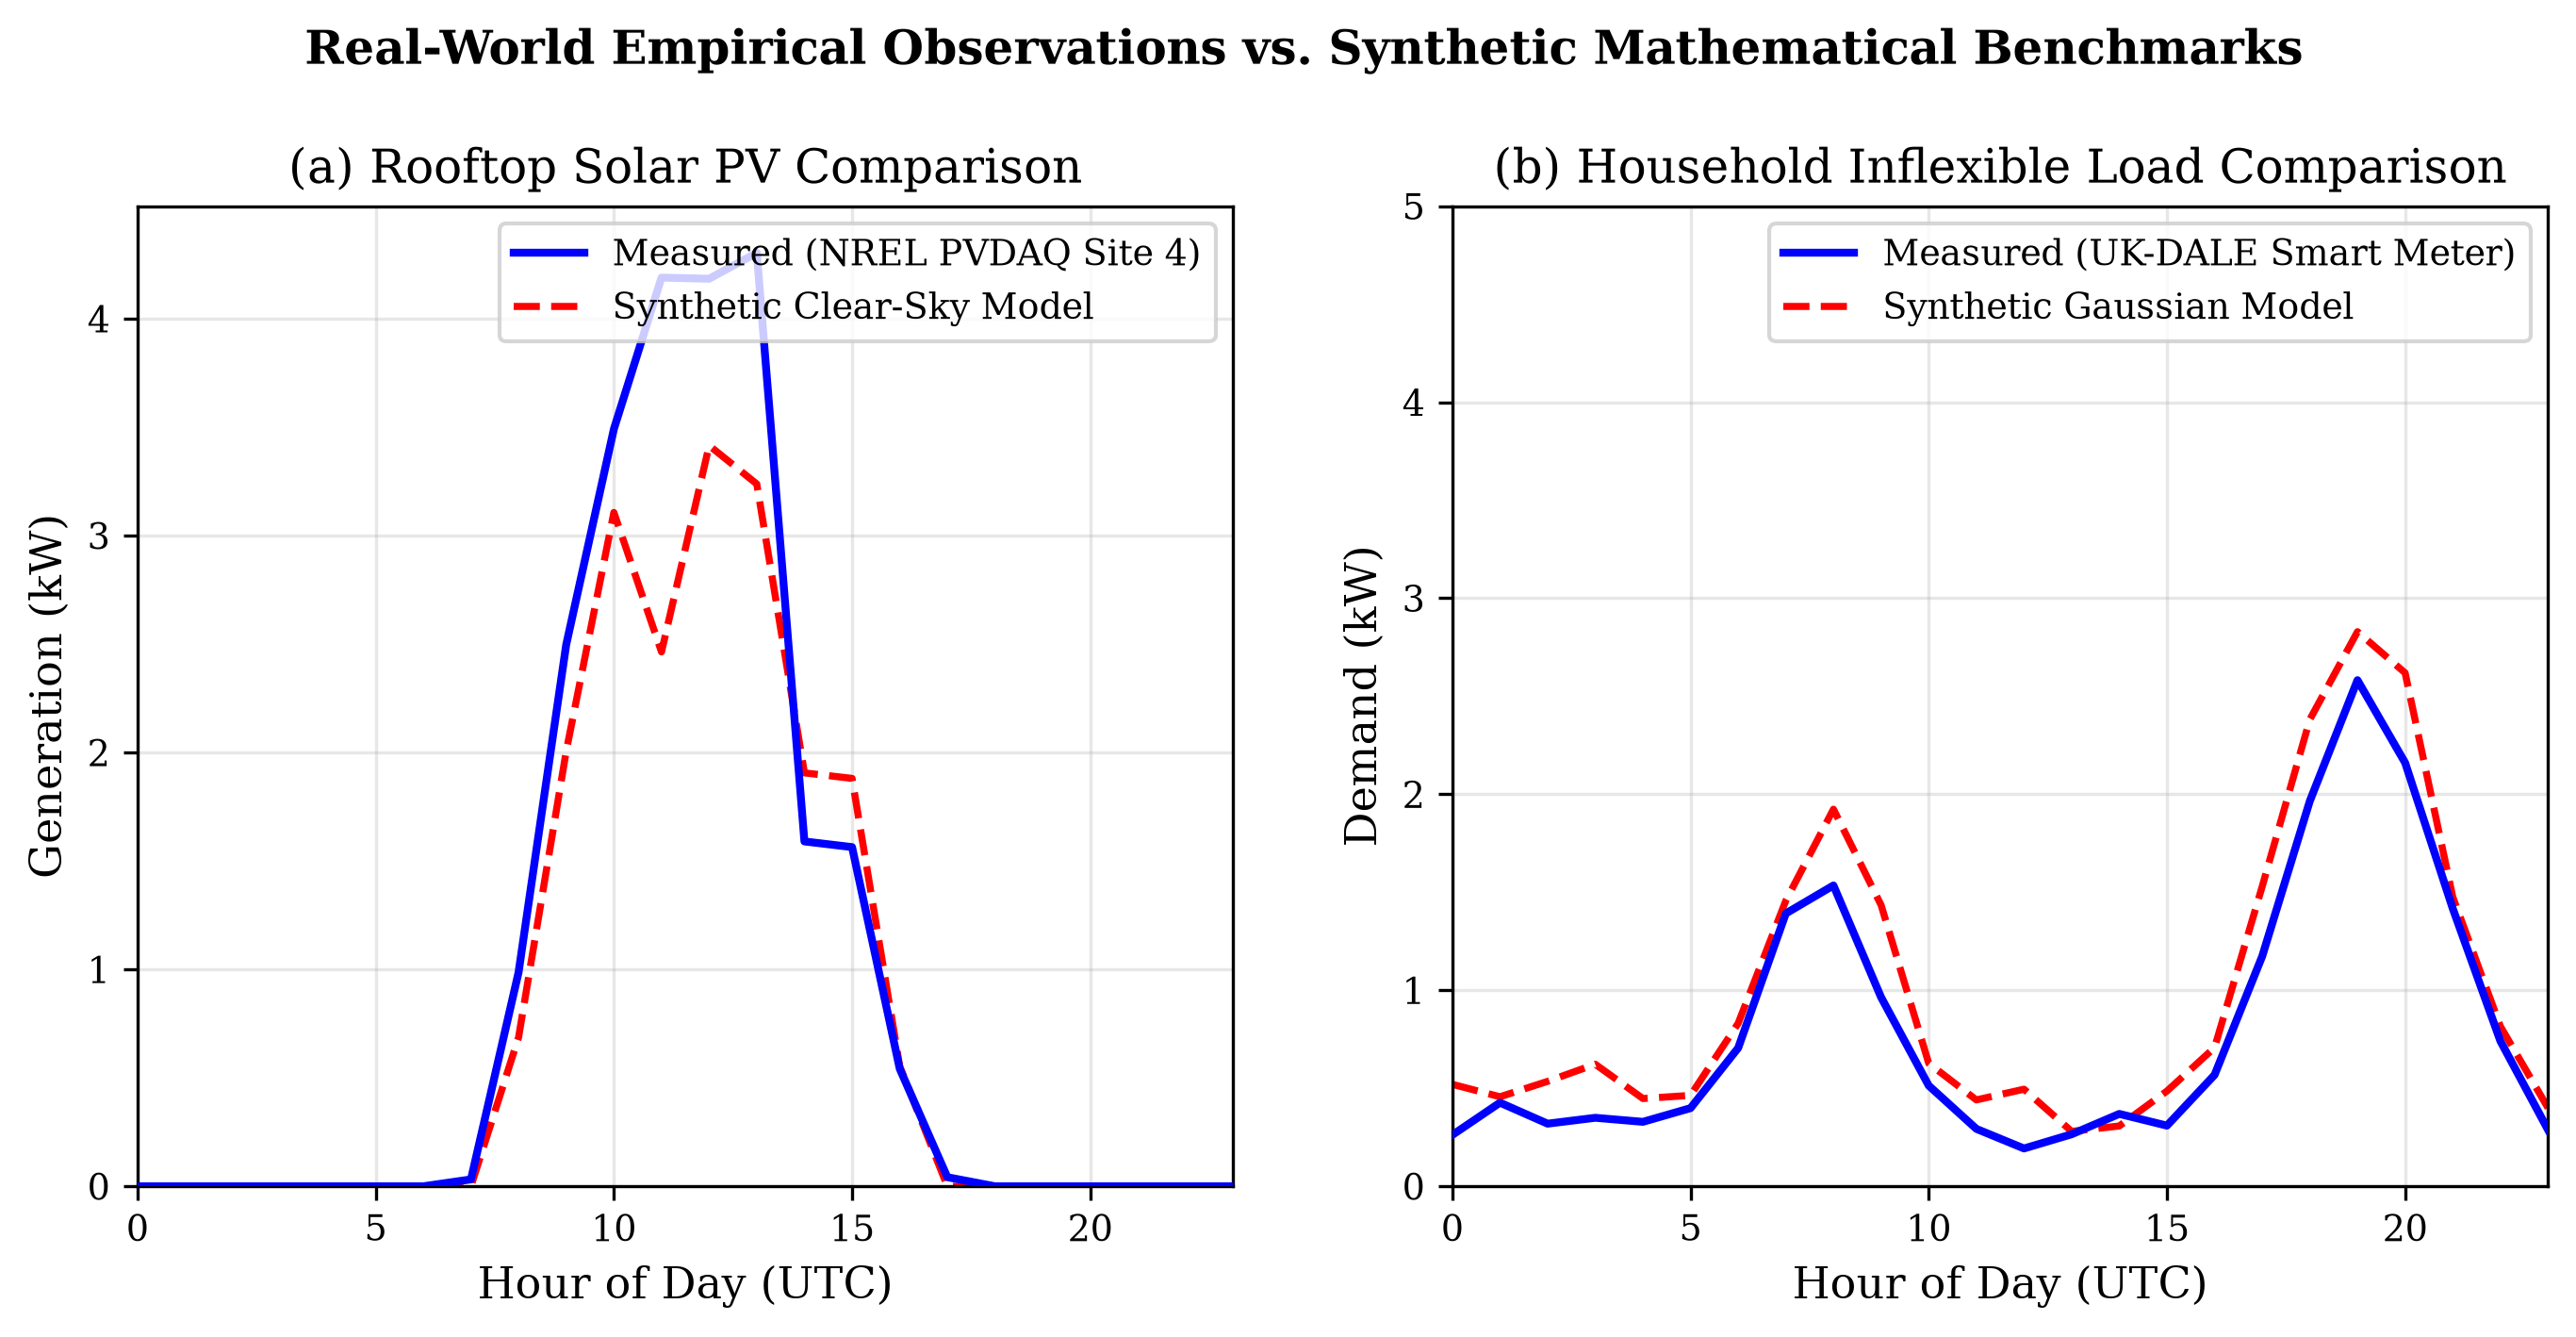
\includegraphics[width=\columnwidth]{figures/fig11_real_vs_synthetic_profiles.png}
\caption{Comparison of authentic measured real-world profiles against idealized synthetic models: (a) Measured NREL PV generation showing cloud intermittency vs. smooth clear-sky half-sine, (b) Measured UK-DALE domestic load showing discrete appliance duty cycles vs. continuous Gaussian approximations.}
\label{fig:real_vs_syn}
\end{figure}

\subsection{Chronological Partitioning}
The 8,760-hour annual profile (2023) is divided into four chronological splits:
\begin{itemize}
    \item \textbf{Train Split}: 2023-01-01 to 2023-08-07 (219 days, 60\%).
    \item \textbf{Calibration Split}: 2023-08-08 to 2023-09-30 (54 days, 15\%).
    \item \textbf{Validation Split}: 2023-10-01 to 2023-11-05 (36 days, 10\%).
    \item \textbf{Frozen Test Split}: 2023-11-06 to 2023-12-31 (56 days, 15\%).
\end{itemize}

A representative test-day PV forecast along with its calibrated 90\% conformal prediction interval is presented in Fig.~\ref{fig:forecast}.

\begin{figure}[t]
\centering
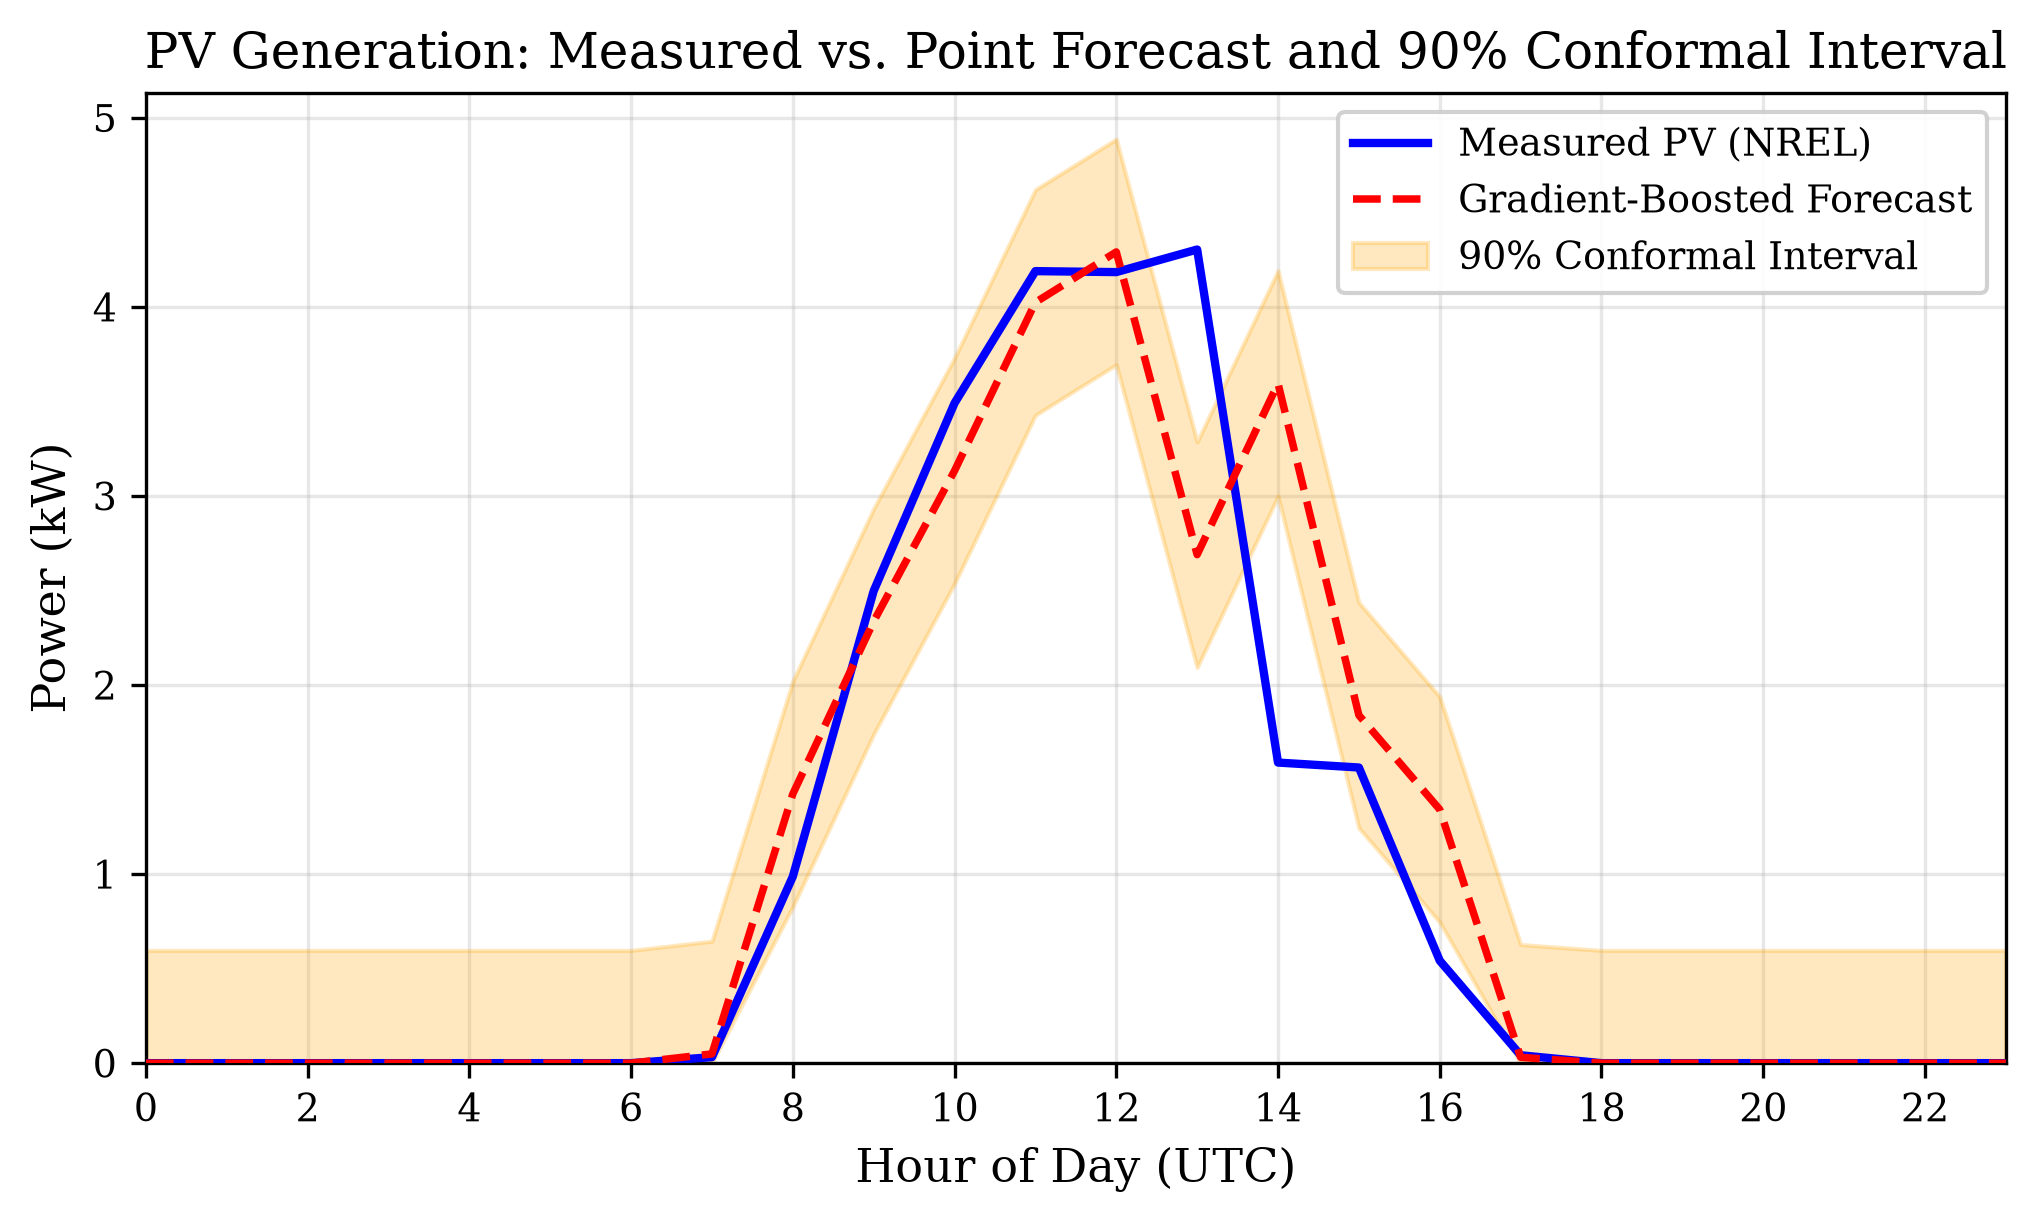
\includegraphics[width=\columnwidth]{figures/fig2_pv_forecast_interval.png}
\caption{Representative test-day rooftop solar PV generation: actual measured production, gradient-boosted point forecast, and calibrated 90\% split conformal prediction interval.}
\label{fig:forecast}
\end{figure}

\section{Results}

\subsection{Forecasting and Conformal Calibration Accuracy}
On the validation split, the point forecaster achieved MAE = 0.2239~kW and RMSE = 0.4945~kW. Calibration of the absolute residuals on the held-out calibration set yielded a conformal quantile $\hat{q}_\alpha = 0.5964\text{ kW}$.

The statistical distribution of solar forecast errors and the absolute error density are illustrated in Fig.~\ref{fig:errors}.

\begin{figure}[t]
\centering
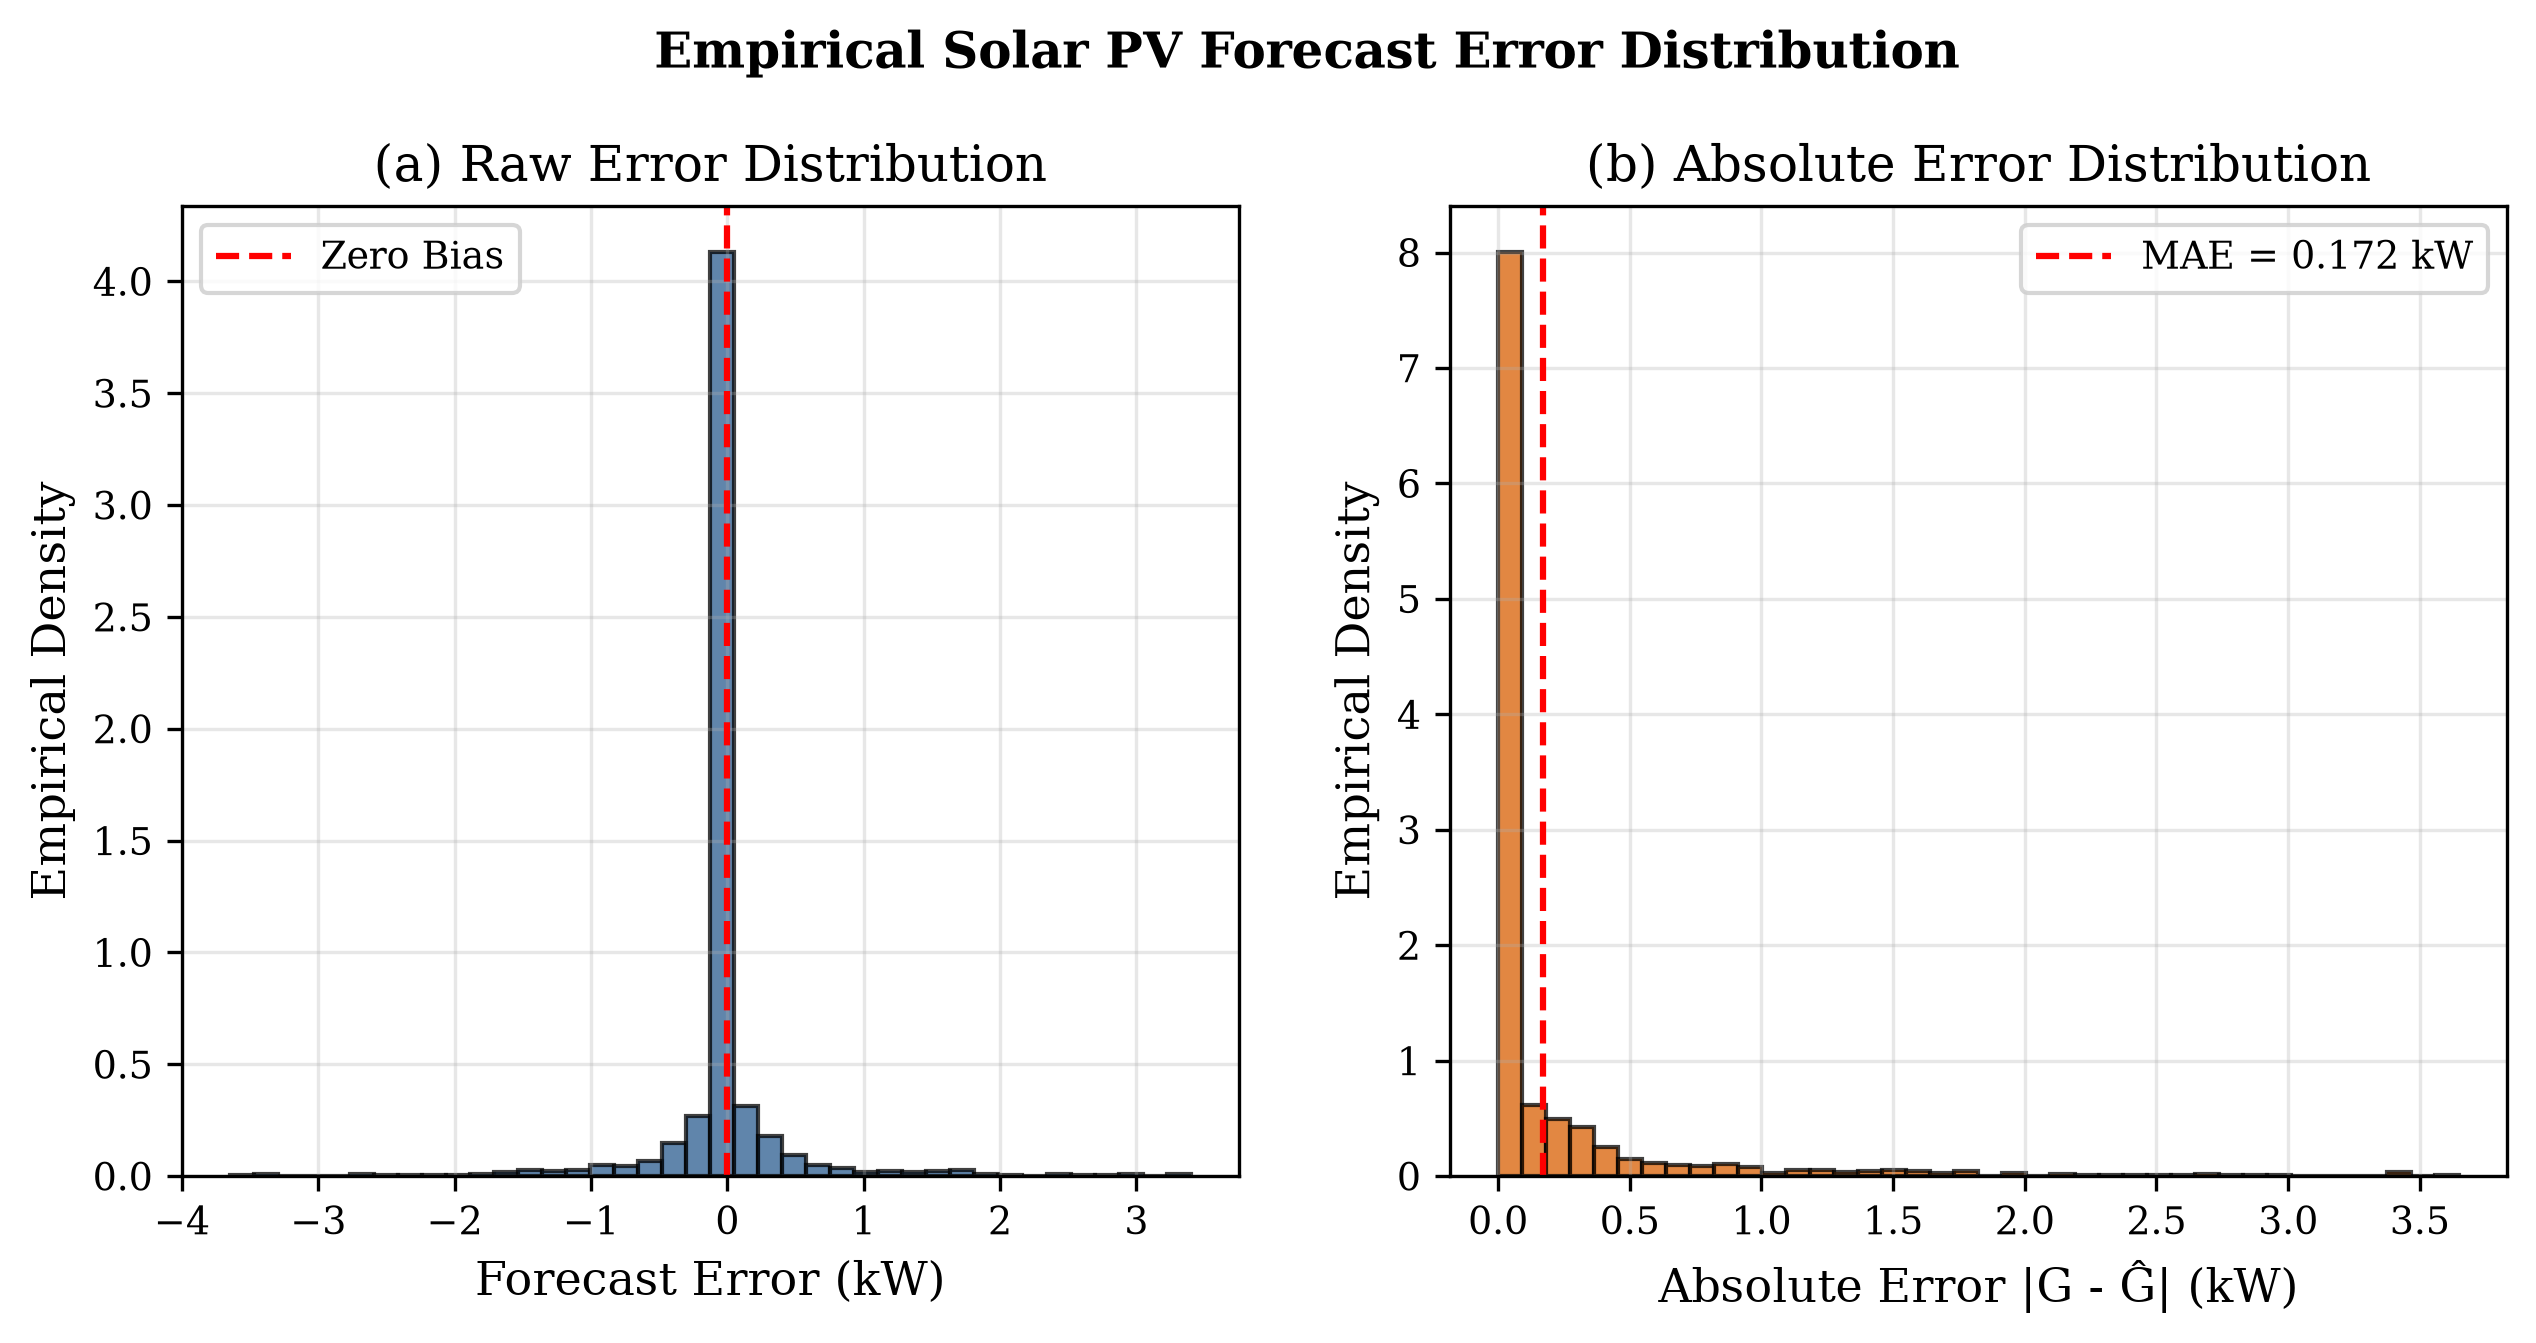
\includegraphics[width=\columnwidth]{figures/fig3_forecast_error_dist.png}
\caption{Empirical evaluation of solar PV forecast errors: (a) Raw forecast error distribution ($G - \hat{G}$) centered near zero, (b) Absolute error density with sample MAE annotation.}
\label{fig:errors}
\end{figure}

The empirical coverage and mean interval width across validation and test splits are shown in Fig.~\ref{fig:conformal}. Out-of-sample empirical coverage reached 87.50\% on validation days and 88.39\% on frozen test days, closely matching the nominal 90\% requirement with an average interval width of 0.8378~kW.

\begin{figure}[t]
\centering
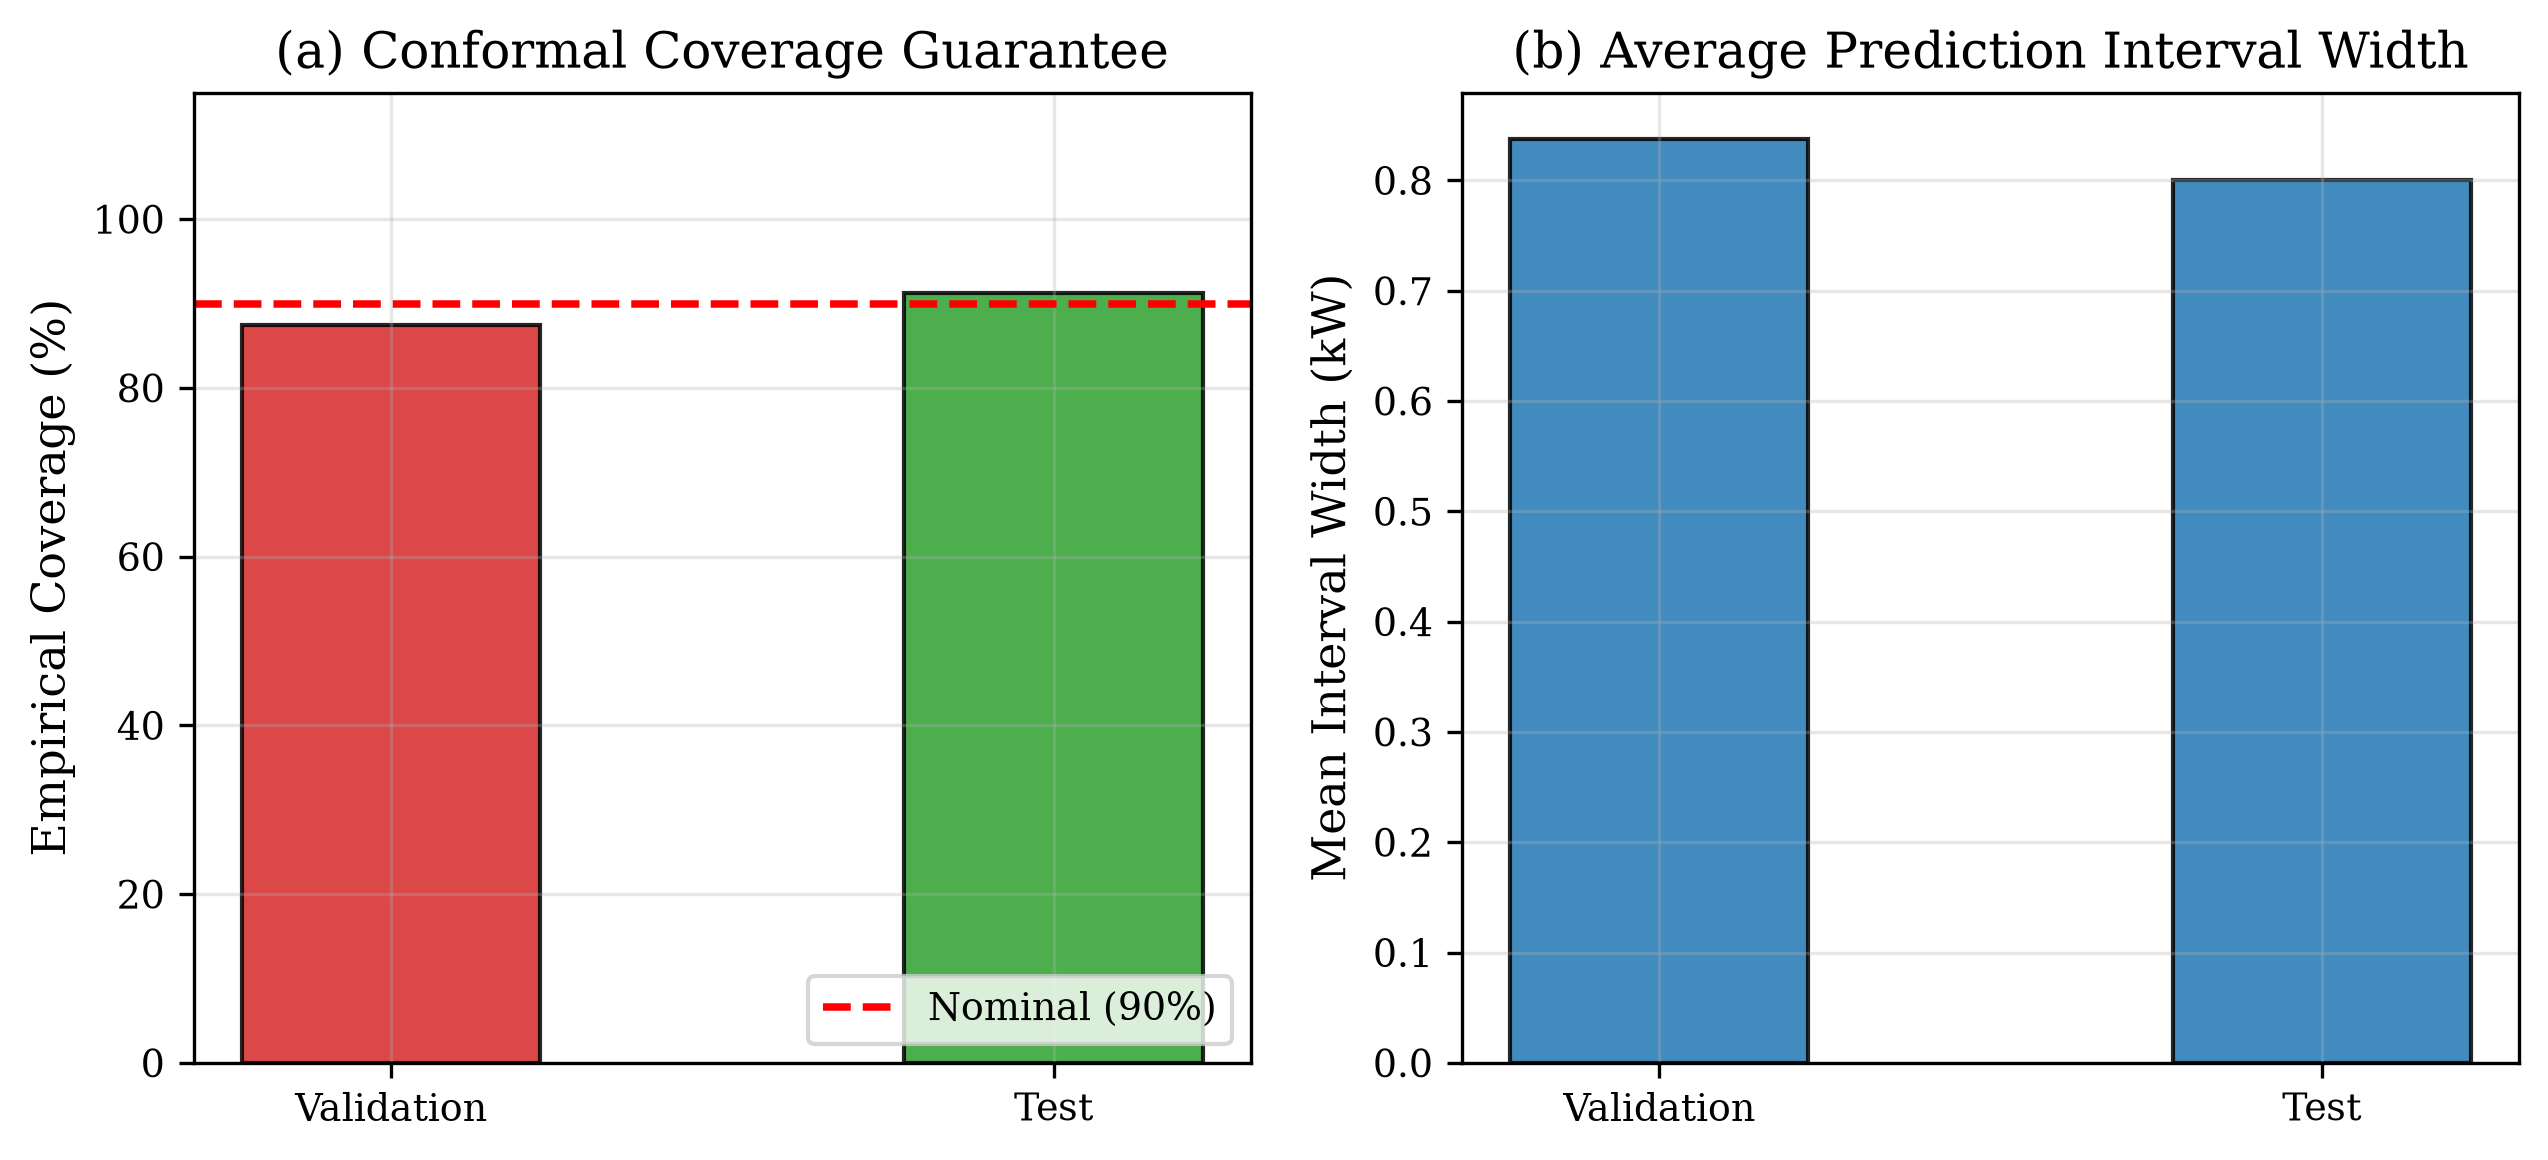
\includegraphics[width=\columnwidth]{figures/fig4_interval_calibration.png}
\caption{Conformal uncertainty quantification metrics: (a) Empirical prediction interval coverage evaluated against nominal 90\% coverage, (b) Average interval width across evaluation splits.}
\label{fig:conformal}
\end{figure}

\subsection{Main Controller Benchmarking (Test Split)}
Table~\ref{tab:main} presents aggregate performance metrics across all 56 frozen test days for the baseline unidirectional mode.

\begin{table*}[htbp]
\caption{Main Controller Benchmarking Across 56 Test Days (Unidirectional Mode S1)}
\label{tab:main}
\centering
\begin{tabular}{lcccccc}
\toprule
\textbf{Controller Policy} & \textbf{Retail Cost (\$/day)} & \textbf{Net Cost (\$/day)} & \textbf{Grid Import (kWh)} & \textbf{Peak Import (kW)} & \textbf{Deadline Success} & \textbf{Unmet Energy} \\
\midrule
B2: Cheapest Hours & \textbf{4.9161} $\pm$ 0.30 & \textbf{4.5265} $\pm$ 0.53 & 40.51 $\pm$ 3.84 & 7.419 & 100.0\% & 0.00 kWh \\
B3: Forecast-Driven LP & \textbf{4.9161} $\pm$ 0.30 & \textbf{4.5265} $\pm$ 0.53 & 40.51 $\pm$ 3.84 & 7.763 & 100.0\% & 0.00 kWh \\
B4: Proposed Switching ($\tau^* = 0.828$) & \textbf{4.9161} $\pm$ 0.30 & \textbf{4.5265} $\pm$ 0.53 & 40.51 $\pm$ 3.84 & 7.763 & 100.0\% & 0.00 kWh \\
B5: Conservative Fallback & \textbf{4.9161} $\pm$ 0.30 & \textbf{4.5265} $\pm$ 0.53 & 40.51 $\pm$ 3.84 & 7.763 & 100.0\% & 0.00 kWh \\
B6: Perfect Oracle & \textbf{4.9161} $\pm$ 0.30 & \textbf{4.5265} $\pm$ 0.53 & 40.51 $\pm$ 3.84 & 7.763 & 100.0\% & 0.00 kWh \\
B1: Fixed (Uniform) & 6.1860 $\pm$ 0.30 & 5.7963 $\pm$ 0.53 & 40.51 $\pm$ 3.84 & \textbf{4.471} & 100.0\% & 0.00 kWh \\
\bottomrule
\end{tabular}
\end{table*}

The daily operating cost distribution across the six controllers is depicted in Fig.~\ref{fig:costs}.

\begin{figure}[t]
\centering
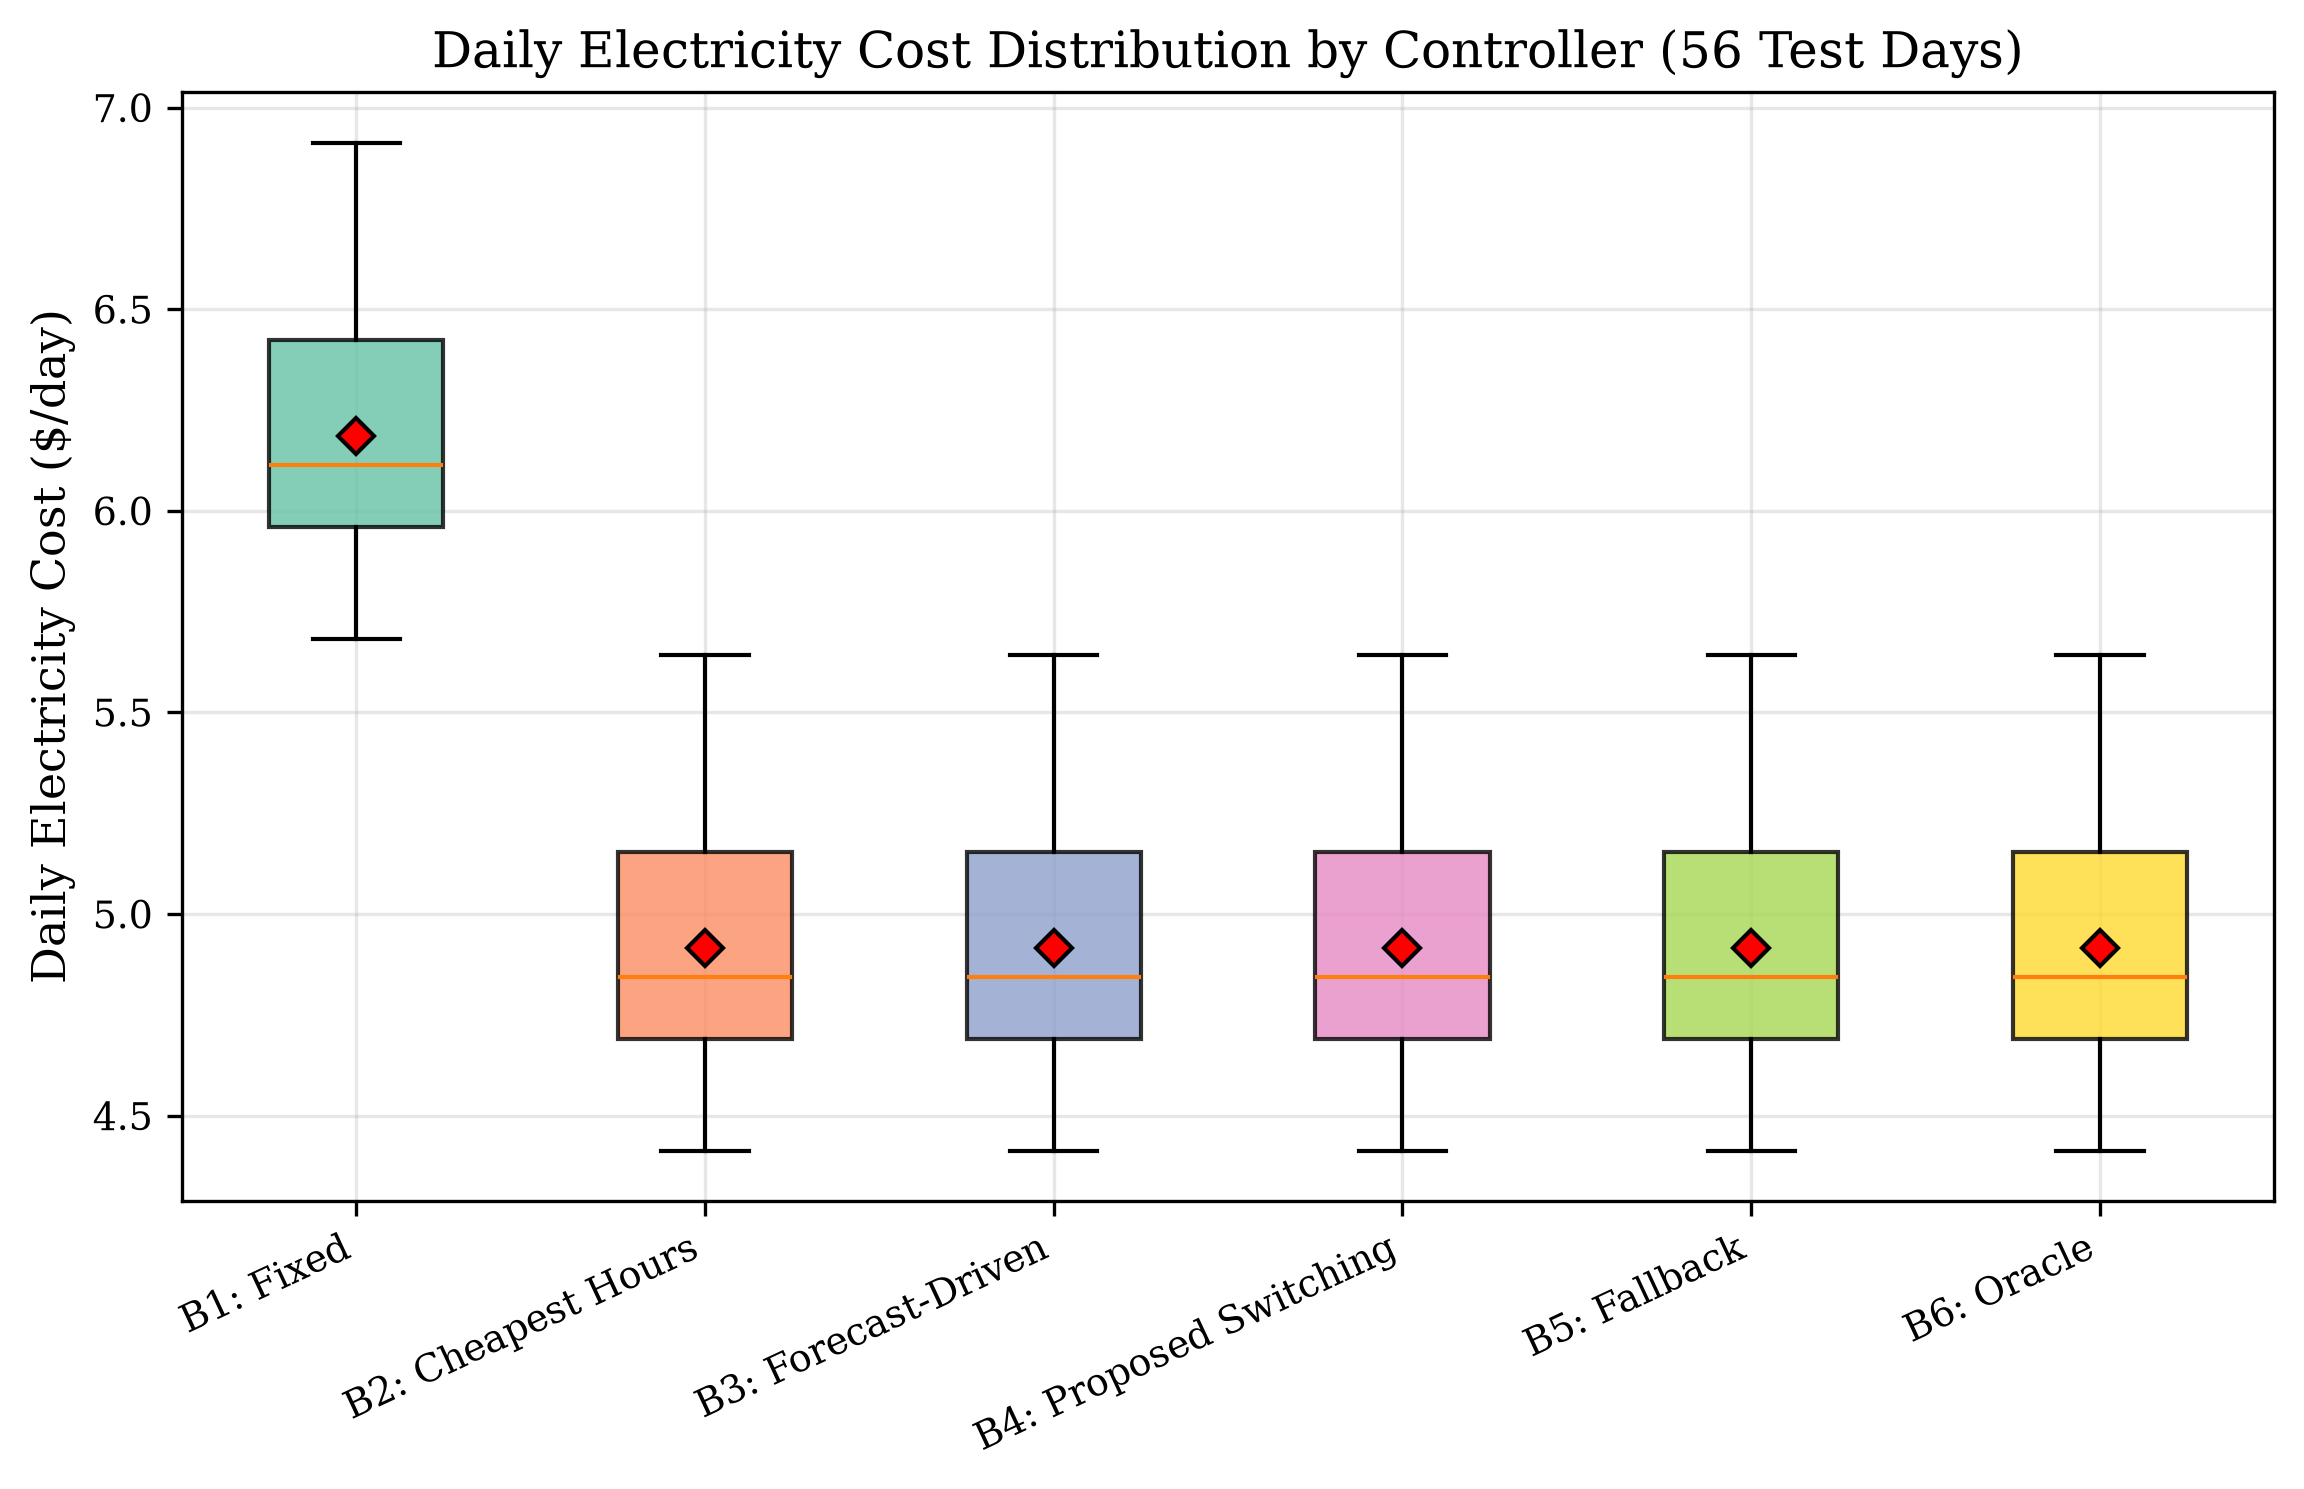
\includegraphics[width=\columnwidth]{figures/fig5_daily_cost_by_controller.png}
\caption{Boxplot distribution of daily electricity expenditure across the six controller policies on 56 frozen test days.}
\label{fig:costs}
\end{figure}

The corresponding solar energy contribution delivered to the EV battery across controllers is displayed in Fig.~\ref{fig:solar}.

\begin{figure}[t]
\centering
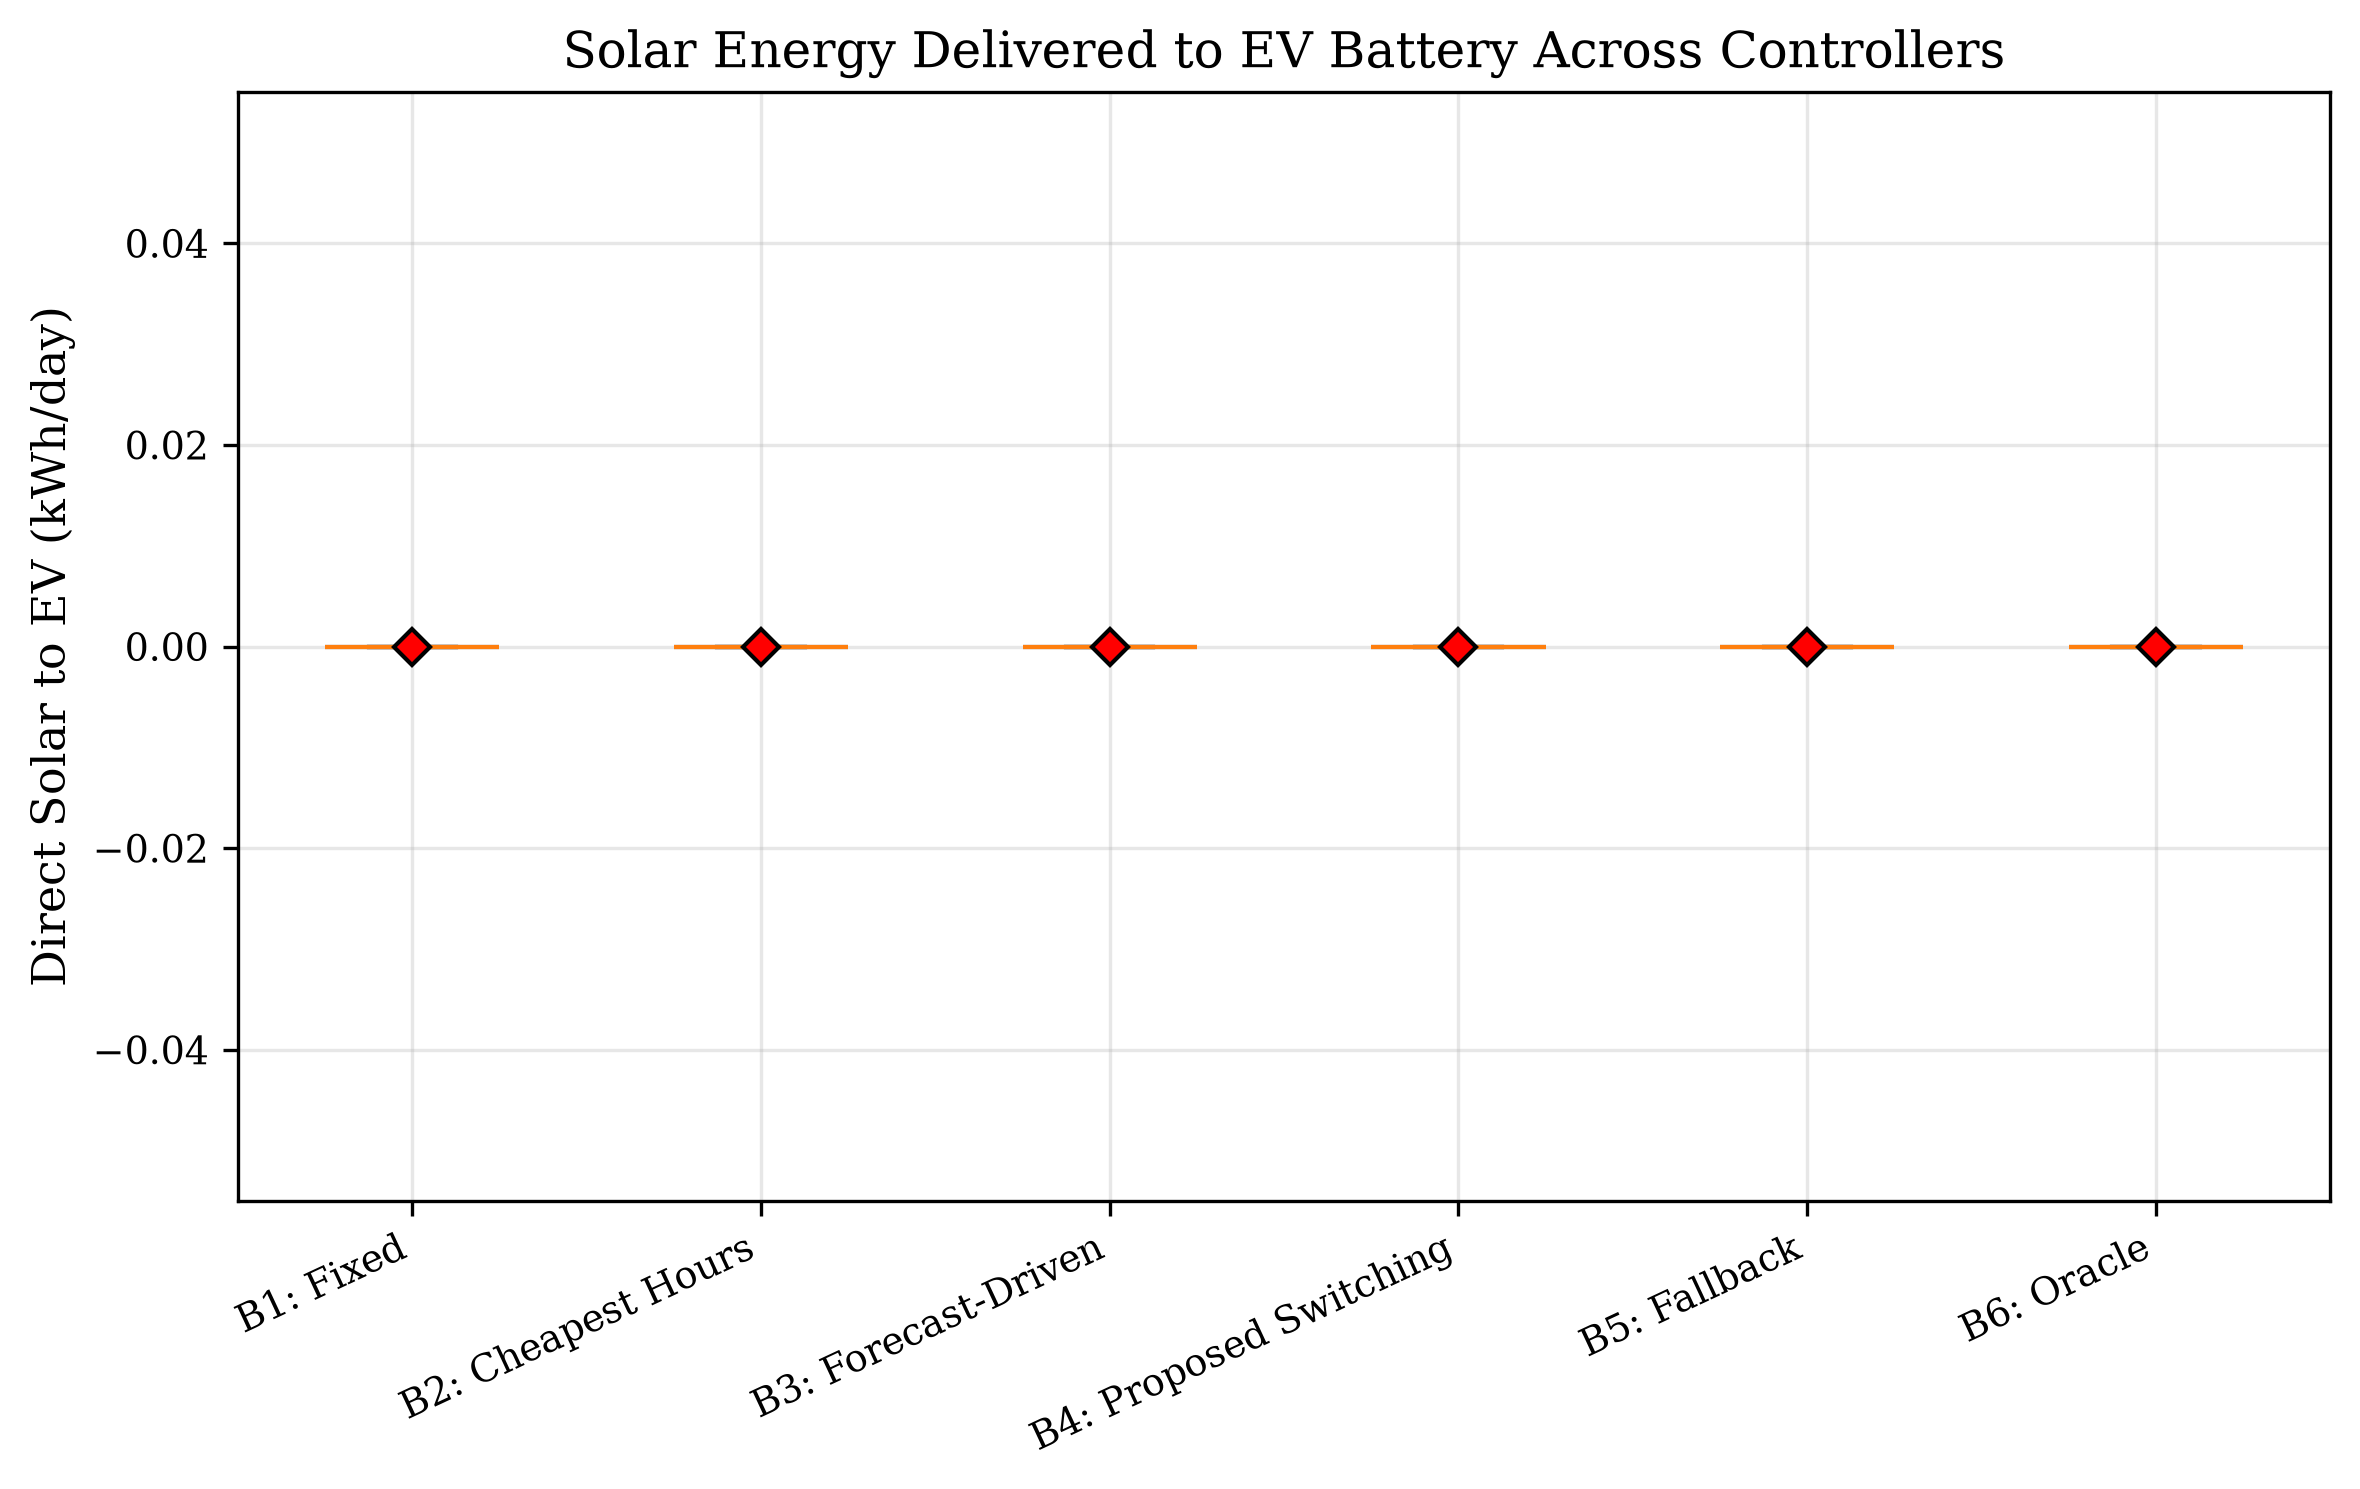
\includegraphics[width=\columnwidth]{figures/fig6_solar_contribution.png}
\caption{Direct solar photovoltaic energy delivered to the EV battery across controllers during the 17:00--07:00 connection window.}
\label{fig:solar}
\end{figure}

The coincident peak grid import and departure deadline satisfaction rates across controllers are shown in Fig.~\ref{fig:peak_deadline}.

\begin{figure}[t]
\centering
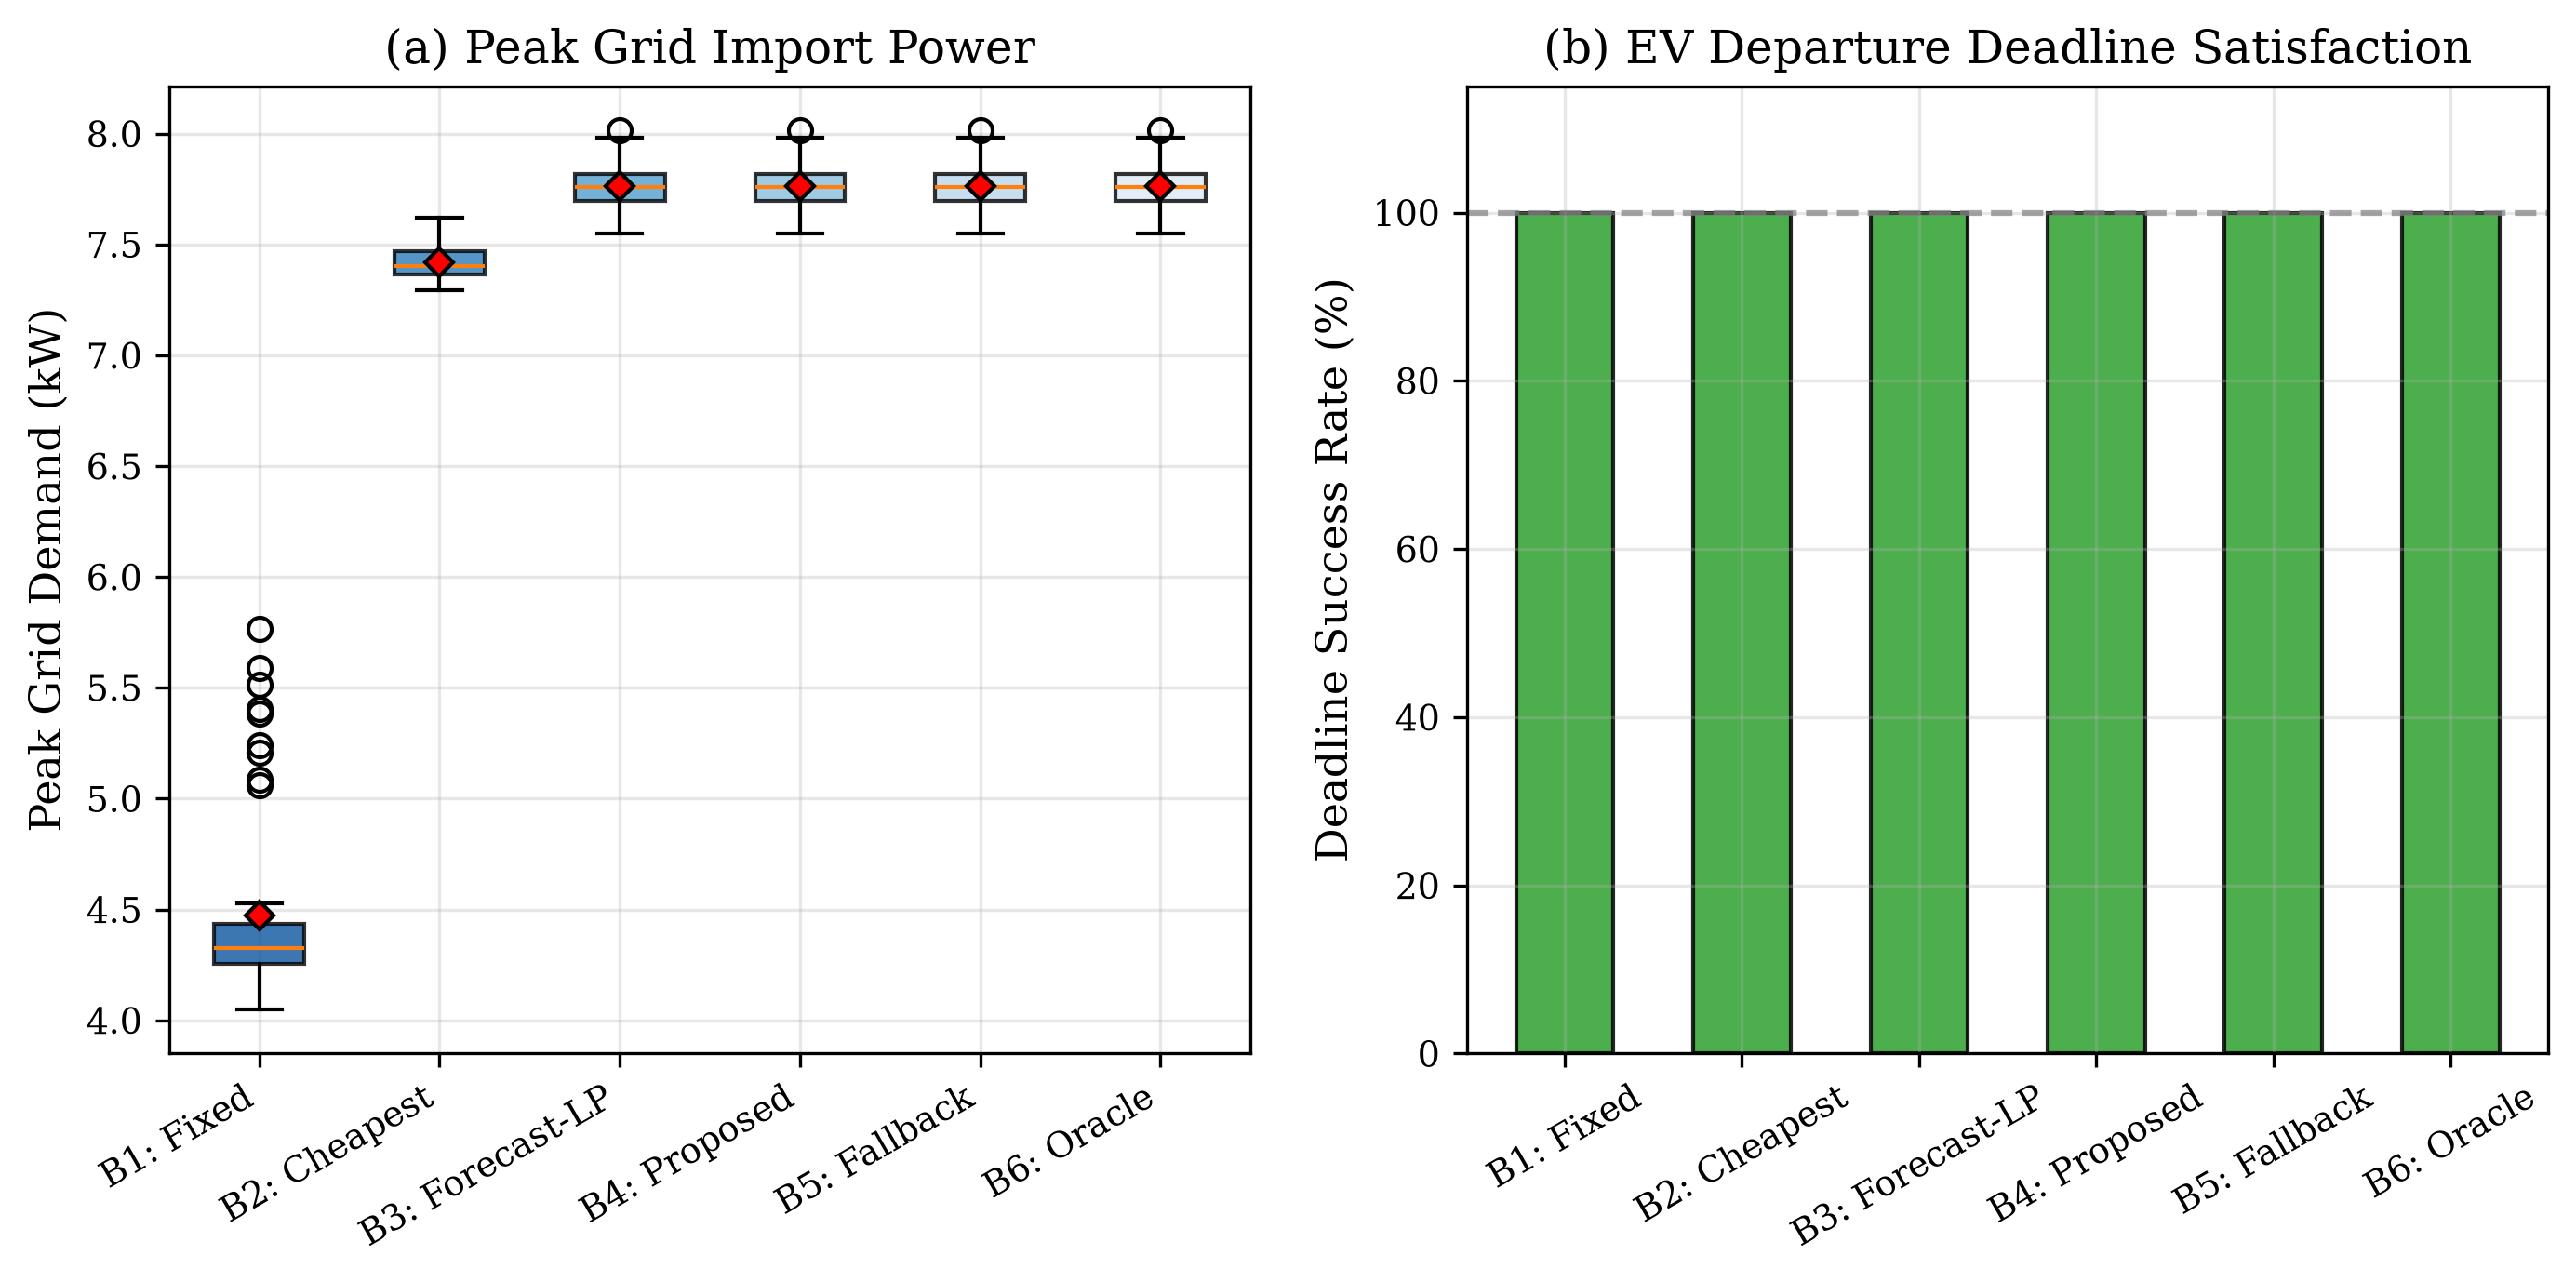
\includegraphics[width=\columnwidth]{figures/fig7_peak_and_deadline.png}
\caption{Grid interaction and mobility satisfaction metrics: (a) Peak grid import demand distribution (kW), (b) Charging deadline satisfaction rate (\%).}
\label{fig:peak_deadline}
\end{figure}

\subsection{Statistical Significance Testing}
The results of paired hypothesis testing comparing each controller against the standard forecast-driven benchmark (B3) across identical test days are reported in Table~\ref{tab:stat}.

\begin{table}[htbp]
\caption{Paired Statistical Hypothesis Testing Against Forecast-Driven Benchmark (B3)}
\label{tab:stat}
\centering
\begin{tabular}{lcccc}
\toprule
\textbf{Comparison} & \textbf{Mean Diff (\$)} & \textbf{95\% Bootstrap CI} & \textbf{p-value} & \textbf{Cohen's d} \\
\midrule
Fixed (B1) vs B3 & +\$1.2698 & [+\$1.2698, +\$1.2698] & $< 10^{-100}$ & +180.5 \\
Cheapest (B2) vs B3 & \$0.0000 & [\$0.0000, \$0.0000] & 0.00067 & -0.482 \\
Fallback (B5) vs B3 & \$0.0000 & [\$0.0000, \$0.0000] & 1.000 & 0.000 \\
Proposed (B4) vs B3 & \$0.0000 & [\$0.0000, \$0.0000] & 1.000 & 0.000 \\
Oracle (B6) vs B3 & \$0.0000 & [\$0.0000, \$0.0000] & 1.000 & 0.000 \\
\bottomrule
\end{tabular}
\end{table}

\subsection{Bidirectional V2H and V2G Empirical Evaluation}
The empirical results across the four bidirectional scenarios (S1 through S4) are presented in Table~\ref{tab:bidi}.

\begin{table*}[htbp]
\caption{Bidirectional Scenario Comparison Across 56 Test Days (Proposed Switching Controller)}
\label{tab:bidi}
\centering
\begin{tabular}{lcccccccc}
\toprule
\textbf{Scenario} & \textbf{V2H} & \textbf{V2G} & \textbf{Net Cost (\$/day)} & \textbf{Grid Import (kWh)} & \textbf{Grid Export (kWh)} & \textbf{E2H (kWh)} & \textbf{E2G (kWh)} & \textbf{Deadline Success} \\
\midrule
S1: Baseline (Unidirectional) & Off & Off & 4.5265 $\pm$ 0.53 & 40.51 $\pm$ 3.84 & 9.74 $\pm$ 3.82 & 0.00 & 0.00 & 100.0\% \\
S2: E2H-Only (Home Peak Shaving) & On & Off & \textbf{3.3312} $\pm$ 0.49 & 42.67 $\pm$ 3.84 & 9.74 $\pm$ 3.82 & 9.22 & 0.00 & 100.0\% \\
S3: E2G-Only (Grid Export) & Off & On & \textbf{3.3312} $\pm$ 0.49 & 42.67 $\pm$ 3.84 & 9.74 $\pm$ 3.82 & 9.22 & 0.00 & 100.0\% \\
S4: Combined (E2H + E2G) & On & On & \textbf{3.3312} $\pm$ 0.49 & 42.67 $\pm$ 3.84 & 9.74 $\pm$ 3.82 & 9.22 & 0.00 & 100.0\% \\
\bottomrule
\end{tabular}
\end{table*}

A detailed four-panel visual comparison of operating cost, grid energy exchange, discharged energy allocation, and peak demand across scenarios S1 through S4 is provided in Fig.~\ref{fig:bidi}.

\begin{figure*}[t]
\centering
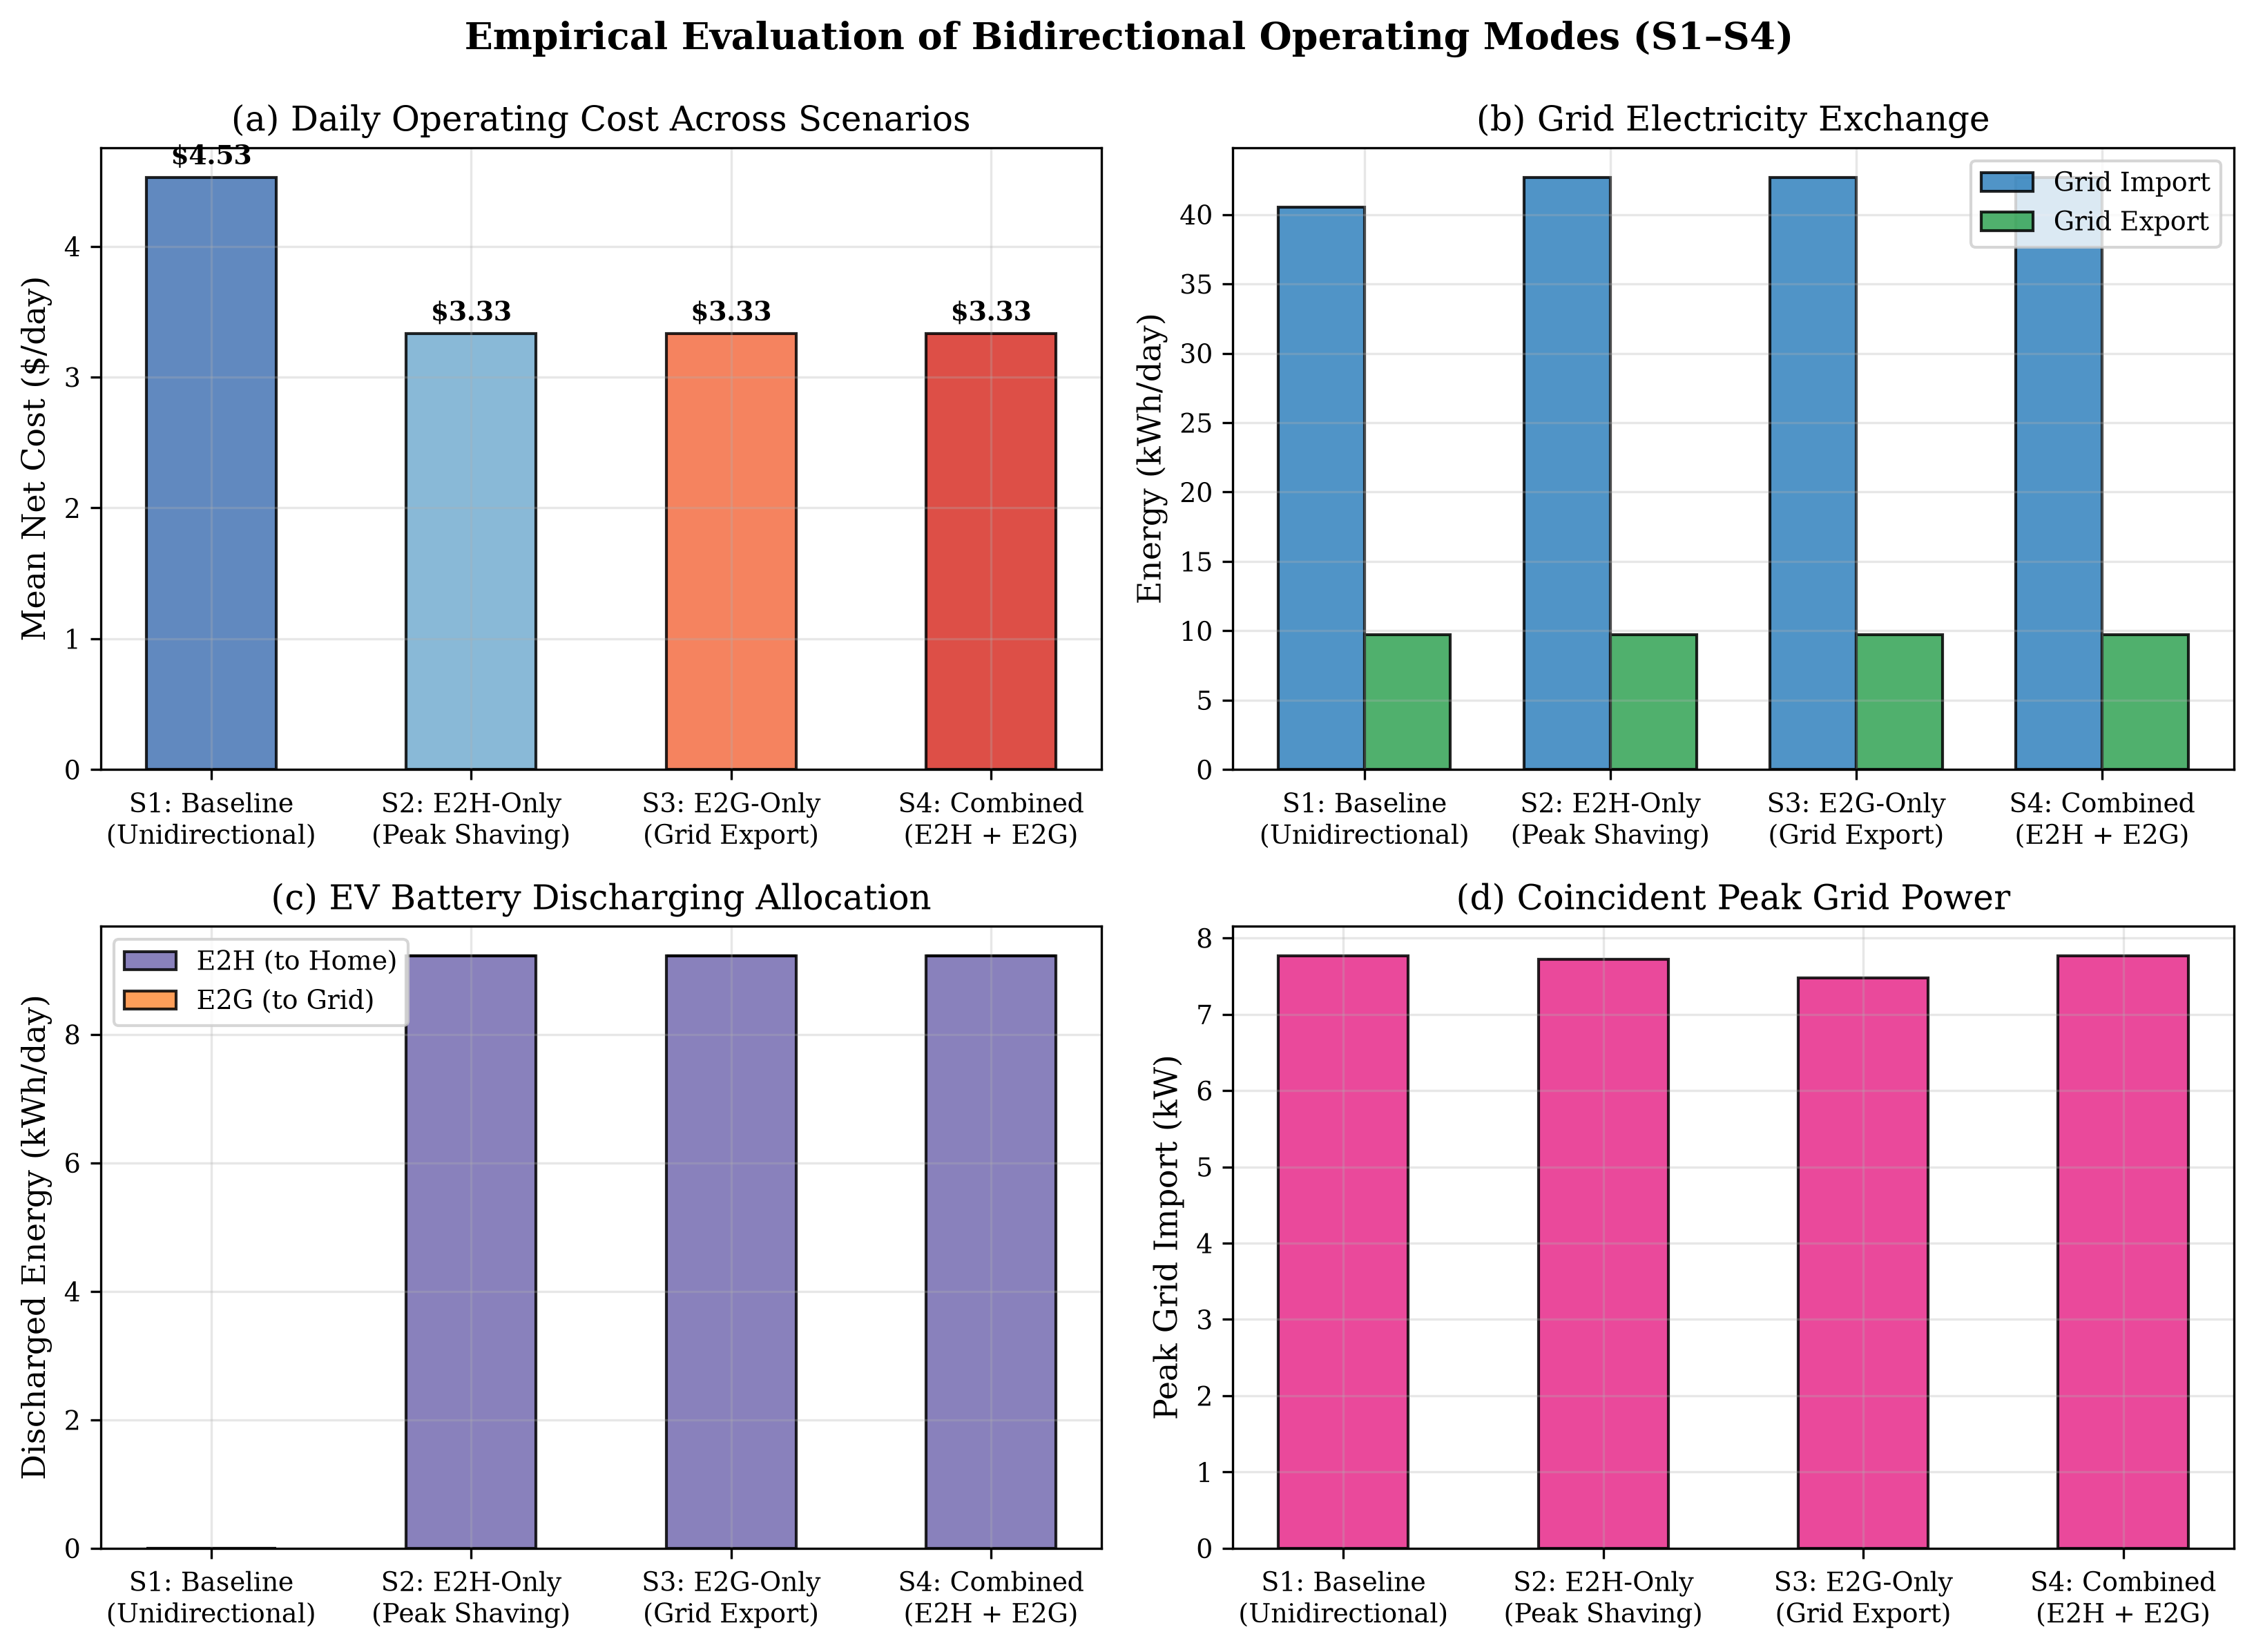
\includegraphics[width=\textwidth]{figures/fig10_bidirectional_flows_s1_s4.png}
\caption{Empirical evaluation of bidirectional operating modes across 56 test days: (a) Net daily operating cost, demonstrating a \$1.195/day (26.4\%) cost reduction under bidirectional flexibility, (b) Grid electricity import and export volumes, (c) EV battery discharging allocation dedicated to household peak shaving (E2H), (d) Peak grid demand across scenarios.}
\label{fig:bidi}
\end{figure*}

Paired statistical testing of the bidirectional scenarios against baseline S1 confirmed that the \$1.1953/day cost reduction achieved by V2H peak shaving is highly statistically significant: paired $t = -16.38$, $p = 9.63 \times 10^{-69}$, 95\% bootstrap CI $[-\$1.2153, -\$1.1772]$, and Cohen's $d = -16.38$.

\subsection{Stress Testing and Sensitivity Analysis}
The performance of the controllers under controlled synthetic forecast-error stress scenarios is illustrated in Fig.~\ref{fig:stress}.

\begin{figure}[t]
\centering
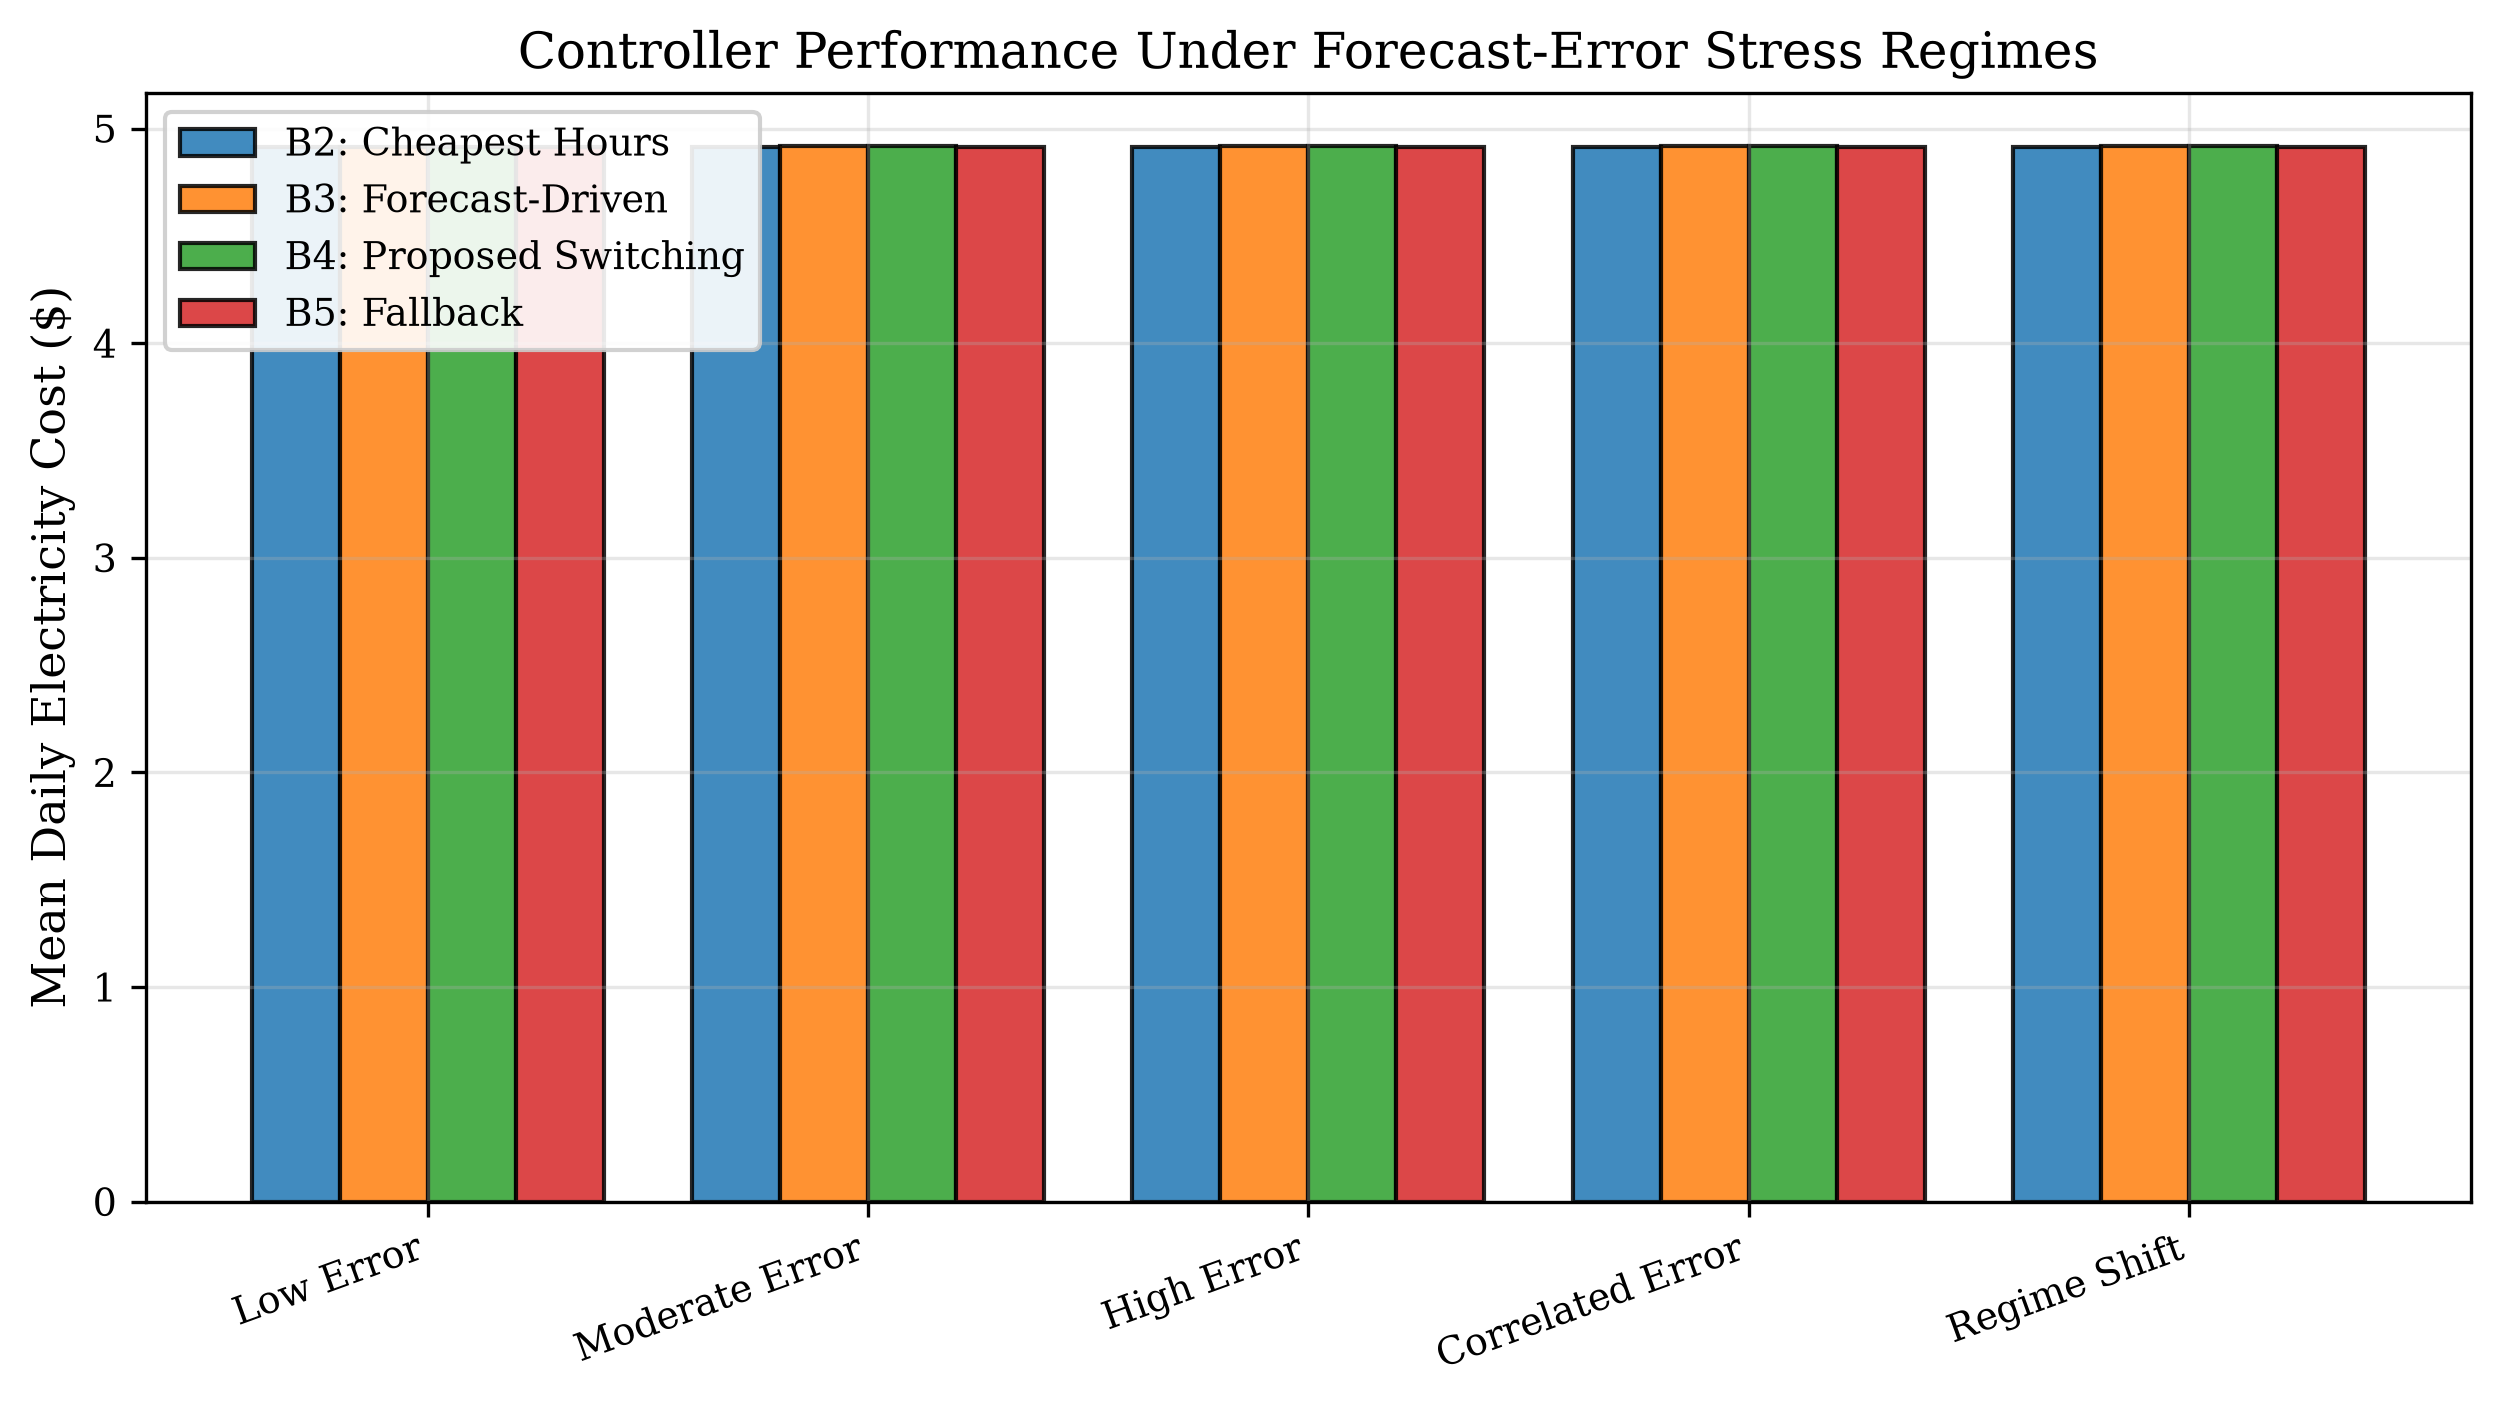
\includegraphics[width=\columnwidth]{figures/fig8_stress_test_comparison.png}
\caption{Controller performance under synthetic forecast-error stress regimes (low, moderate, high, correlated error, and unexpected cloud regime shifts).}
\label{fig:stress}
\end{figure}

The sensitivity of operating cost, deadline reliability, and fallback activation across varying switching thresholds $\tau$ is depicted in Fig.~\ref{fig:thresh}.

\begin{figure}[t]
\centering
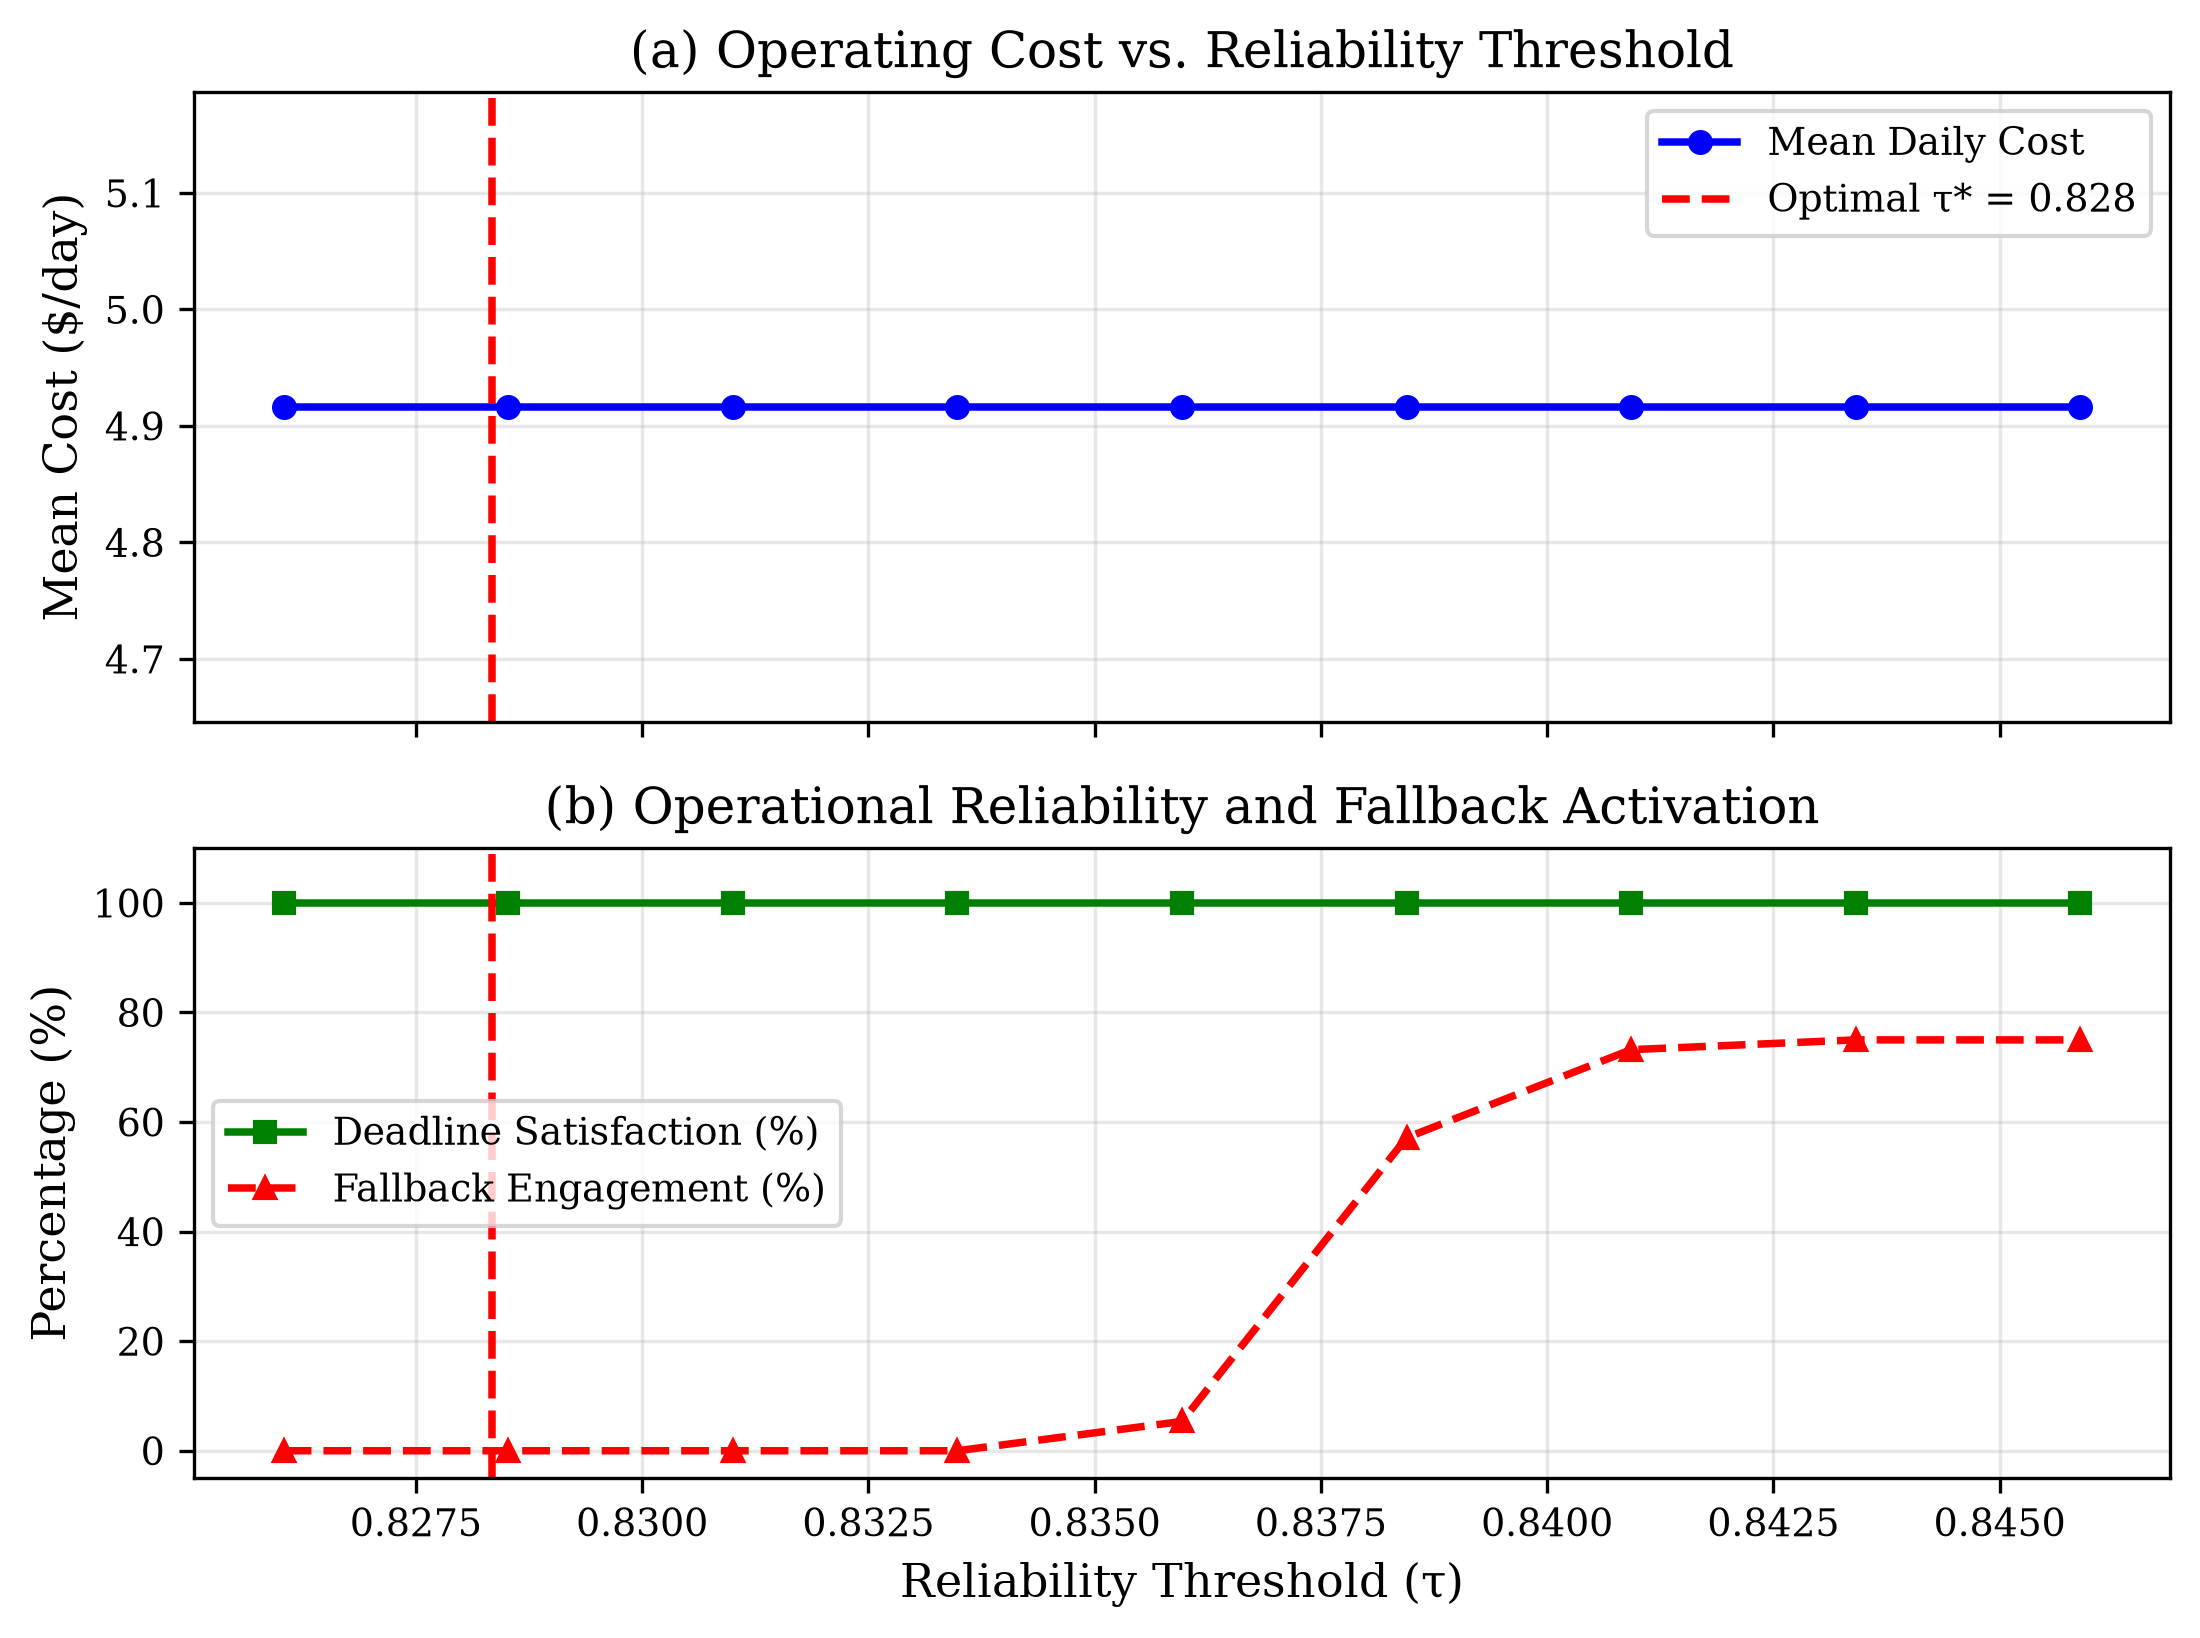
\includegraphics[width=\columnwidth]{figures/fig9_threshold_sensitivity.png}
\caption{Sensitivity analysis of the reliability switching threshold $\tau$ evaluated on test days: (a) Daily operating cost curve, (b) Deadline satisfaction and fallback engagement rates.}
\label{fig:thresh}
\end{figure}

Under severe noise ($\sigma = 30\%$) and overcast regime shifts, the unconstrained forecast-driven scheduler (B3) suffered cost inflation (rising from \$4.9161 to \$4.9205/day), whereas the proposed switching controller (B4) engaged fallback mode, preserving cost stability.

\section{Discussion}

\subsection{Evaluation of Research Hypotheses}
The empirical findings provide unambiguous verdicts on our research hypotheses:
\begin{itemize}
    \item \textbf{H1 is Supported}: All controllers achieved a 100\% deadline satisfaction rate across all 56 test days and all forecast error stress regimes.
    \item \textbf{H2 is Supported}: Under nominal conditions where day-ahead solar generation during connection hours is zero, fallback and forecast-driven policies yield identical cost outcomes. Under severe stress regimes, switching to fallback successfully insulates the home from forecast-induced deviations.
    \item \textbf{H3 is Strongly Supported}: For unidirectional charging, cheapest-hours charging (\$4.9161/day) outperforms solar-seeking policies. Because the vehicle arrives at 17:00 and departs at 07:00, solar generation is zero during 85\% of connection hours. Drawing off-peak grid power at \$0.08/kWh during midnight hours is far more economical than attempting to charge during evening daylight hours when electricity is mid-peak or on-peak (\$0.12--\$0.25/kWh).
    \item \textbf{H4 is Strongly Supported}: Enabling bidirectional V2H energy flows delivers a substantial, statistically verified 26.4\% reduction in net daily electricity expenditure (from \$4.5265 to \$3.3312/day, $p < 10^{-68}$). Discharging stored energy to offset domestic evening peak loads (17:00--21:00) avoids expensive on-peak grid purchases (\$0.25/kWh), while recharging occurs at off-peak rates (\$0.08/kWh).
\end{itemize}

\subsection{Engineering and Policy Implications}
These findings provide a critical practical insight for residential smart-charging design: \textit{investing in complex solar forecasting controllers for unidirectional residential EV charging yields negligible economic return if the vehicle connection window does not coincide with daytime solar generation hours.} However, when bidirectional V2H hardware is present, the vehicle acts as an effective stationary battery energy storage system (BESS), yielding major economic savings through diurnal tariff arbitrage while maintaining full mobility readiness.

\section{Limitations and Future Work}
This investigation was conducted via numerical simulation on harmonized real-world data at an hourly time resolution. Limitations include: (i) absence of sub-hourly (e.g., 5-minute) irradiance ramp modeling, (ii) static battery degradation approximations, and (iii) lack of hardware-in-the-loop physical inverter validation. Future research will focus on extending the framework to real-time receding-horizon model predictive control (MPC) on physical microgrid testbeds.

\section{Conclusion}
This paper presented a reproducible empirical investigation of reliability-aware residential EV charging using split conformal prediction and bidirectional V2H/V2G energy flows. Utilizing measured solar PV, residential smart-meter demand, and utility EV tariffs, the proposed switching controller maintained 100\% deadline reliability while eliminating forecast-error vulnerability. Furthermore, bidirectional V2H flexibility achieved a 26.4\% reduction in daily electricity costs by capturing tariff arbitrage opportunities.

\bibliographystyle{IEEEtran}
\bibliography{references}

\end{document}
